\chapter{Debugging Long Infection Chains with Interactive Dynamic Slicing}
\label{sec:ids}

\todo{"Our studies also suggest that developers find concrete values essential for interpreting program state" \cite{ko07:information_needs_in_collocated}}
\todo{collaborative, sharing execution \cite{ko07:information_needs_in_collocated}}
\todo{interactive, navigation, \cite{storey99:cognitive_design_elements}}

% context
Improvements in manual debugging, such as back-in-time debugging, allow developers to debug a program more efficiently in general, but do not assist developers in finding code related to a specific problem.
\Acf{afl} techniques, such as spectrum-based fault analysis or slicing \todo{cite}, can help developers to locate faults by suggesting relevant code locations.
However, developers still need to manually debug the code to identify erroneous state at the suggested locations.
Furthermore, many \ac{afl} tools generate a lot of knowledge about a program's execution in order to find the most helpful suggestions, but then discard this knowledge after the result has been produced.
Not only are developers left with no explanation why a certain code location was considered relevant, but there is also no way to search the vast body of knowledge for helpful insights.

% problem
In large and complex applications, the length of the infection chain, i.e., the distance between the code location of the observed failure and the actually defective code, can be very long.
This reduces the effectiveness of \ac{afl} approaches and makes manual debugging more tedious and time-consuming.
With growing program size, \ac{afl} approaches also often become relatively slow.
While it still may be feasible for developers to run AFL tools to gain initial suggestions on where to start a debug session, the expected waiting time can discourage the use of \ac{afl} tools during debugging.

% contribution
To better help developers debugging long infection chains, we propose to combine automated and manual debugging techniques in a single debugging tool. 
By combining the benefits of both approaches, we expect a synergy that allows for more effective debugging of long infection chains than with two independent tools.

In our work, we combined back-in-time debugging with dynamic slicing.
Our contributions in this field are threefold:
\begin{itemize}
	\item A new configurable slicing algorithm allows quick and iterative refinement of the slicing criteria to adapt the slice to changing developer questions.
	Developers can formulate their question by choosing from different dependency types that will change the outcome of the slice.
	\item The \emph{Slice Navigator} is a UI component that bundles access to the debugger and the slicer.
		It provides context for the current instruction by showing relevant parts of the slice, allows developers to iteratively refine the slicing criteria, and serves as an alternative to breakpoints and stepping.
	\item The integration of dynamic analyses directly in the debugger not only reduces interruptions in developer flow by minimizing context switches between tools and shortens waiting time as recorded run-time data can be re-used; it also allows for a new debugging workflow where developers can isolate a bug by iteratively slicing away correct code.
\end{itemize}
Furthermore, we conducted a user study that suggests less time is needed to follow an infection chain with the Slice Navigator than with traditional or back-in-time debuggers.

\section{Better Slices with Iterative Criteria Refinement}

Modularization is the art of breaking large software into smaller pieces of related code.
If done right, it can greatly improve the maintainability of an application.
Many approaches, such as name spaces or object-oriented programming, were developed to help to structure a program.

Typically, modularization is used to group code that is semantically related.
However, research has shown that developers also break programs down into pieces of code that are related by data flow~\cite{weiser82:programmers_use_slices_when}.
Such "slices" are often not contiguous and can contain code from many different parts of an application, increasing the navigation overhead for developers trying to understand the program.
Here, tools can help to identify related statements, saving time and reducing the mental overhead for developers.

\subsection{Configurable Slicing}

Motivation: continue where \nameref{sec:evolution_of_slicing} stopped.

To determine which statements belong to a slice and which do not, the slicer has to perform a dependency analysis on the program.
Many different approaches exist to conduct such analyses~\cite{korel98:dynamic_program_slicing_methods, tip94:a_survey_of_program}. 
In our work, we used the popular approach of computing dependence graphs.

Static slicing algorithms typically use \emph{\acp{pdg}}, where every node is statement or instruction and directed edges indicate dependency relations~\cite{weiser81:program_slicing}.
For dynamic slicing, the slice precision can be improved by using \emph{\acp{ddg}}, in which each node represents the execution of a statement.
To compute \acp{ddg}, Agrawal \etal\ and Zhang \etal\ developed algorithms that first compute a \ac{pdg} and then combine it with a recorded execution trace~\cite{agrawal90:dynamic_program_slicing,zhang03:precise_dynamic_slicing_algorithms}.
Then, from the \ac{ddg} the slice is derived as a sub-graph.
While this approach produces precise results, it typically takes a long time to complete.
Thus, they also developed multiple algorithms that provide different trade-offs between runtime and precision.


TODO: formal definition of configurable slicing,

\subsection{An Efficient Incrementally Configurable Slicing Algorithm}

We present a new efficient algorithm that produces slices with a very high precision.
Like previous approaches, we derive the slice from a \ac{ddg}, which is computed by combining \acp{pdg} with execution traces.
However, our algorithm has three novel properties that distinguish it from previous solutions.

Firstly, our algorithm avoids unnecessary pre-processing.
Instead of tediously computing a \ac{pdg} of the entire program, small \acp{pdg} are quickly computed on the method-level when needed.
Furthermore, the \ac{ddg} and the slice are built together, constructing only as much of the \ac{ddg} as is required to compute the slice.
This allows the algorithm to work very efficiently, especially when computing small slices in large programs.

Secondly, developers can specify more detailed slicing criteria.
Instead of just selecting statements as a starting point for the slicing, developers can choose to include or exclude different dependency types.
This allows them to narrow down the slice for specific questions, such as "How was this value computed?" or "Why was this line reached?".
Furthermore, disabling all dependency types for a node turns it into a negative criterion.
This way, developers can remove segments of the program that are not of interest.
Slices with negative criteria are no longer technically "accurate", but have much higher precision with respect to the developer's debugging problem.

Thirdly, our algorithm supports iterative modification of the slicing criteria.
Most slicing algorithms take the input, run for a few seconds, and then present the result and terminate.
However, as developers debug the slice, their questions and understanding of the program change.
At this point, computing a new slice would be necessary, but the interruption imposed by the waiting time can break the developer's flow.
Caching the \ac{pdg} or \ac{ddg} can only partially address this problem.
Our algorithm supports quickly changing a previously computed slice by adding, changing, or removing slicing criteria.
This not only increases the overall usefulness of slicing for debugging, but it also allows developers to take full advantage of the fine granularity with which slicing criteria can be specified for our algorithm.

%Inter-method dependencies, i.e., field access, exception control flow, and virtual method call dependencies, are incomplete in these \acp{pdg}.
%When constructing the \ac{ddg}, they will be resolved using the execution trace.
%
%Previous "accurate" dynamic slicing algorithms based on \acp{ddg} work by first building a complete \ac{ddg} and then deriving the slice as a subgraph~\cite{agrawal_90_dynamic_program_slicing,zhang_03_precise_dynamic_slicing_algorithms, wang_08_dynamic_slicing_on_java}.
%Our algorithm builds 
%Since the method-level \acp{pdg} that form the foundation for the \ac{ddg} are also computed on demand only, 

In the next subsection, we describe how the method-level \acp{pdg} are computed.
After that, we show how they are combined with an execution trace to build the \ac{ddg} and the slice, and how incremental changes are applied.
Throughout the remainder of this section, we use a small example to illustrate the slicing algorithm.
\Cref{lst:countLetters} shows a Java method that counts the length of words in a comma-separated word list.
The test in \cref{lst:testCountLetters} checks if the resulting ´long´ array contains correct values.
The code contains no bugs; nevertheless, a developer might choose to slice on the ´assertEquals´ invocation in line 8 to understand how the given input leads to the expected values.

\begin{lstlisting}[float,caption={A method to count letters in a word list.},stepnumber=2,numberfirstline=false,label=lst:countLetters,language=Java]
    public long[] countLetters(String wordList) {
        String[] words = wordList.split(",");
        long[] result = new long[words.length];
        for (int i = 0; i < words.length; i++) {
            String trimmed = words[i].trim();
						result[i] = trimmed.length();
        }
        return result;
    }
\end{lstlisting}

\begin{lstlisting}[float,caption={A test for countLetters.},stepnumber=2,numberfirstline=false,label=lst:testCountLetters,language=Java]
    public void testCountLetters() {
        String input = " hello , all ";
        long expected1 = 5;
        long expected2 = 3;
        long[] result = countLetters(input);
        assertEquals(2, result.length);
        assertEquals(expected1, result[0]);
        assertEquals(expected2, result[1]);
    }
\end{lstlisting}

%
%\begin{lstlisting}[firstnumber=54,float,caption={A test in TimeIntervalParserTest.java},stepnumber=2,label=lst:test]
    %@Test
    %public void testParse3() {
        %String input = " 10h49m789 , 12h ";
        %long expected1 = 10 * 3600000 + 49 * 60000 + 789;
        %long expected2 = 12 * 3600000;
        %Long[] result = new TimeIntervalParser().parse( input );
        %assertEquals( 2, result.length );
        %assertEquals( expected1, result[0].longValue() );
        %assertEquals( expected2, result[1].longValue() );
    %}
%\end{lstlisting}
%
%\begin{lstlisting}[firstnumber=34,float,caption={The method under test, implemented in TimeIntervalParser.java},stepnumber=2,label=lst:parse]
    %public Long[] parse(String paramText) {
        %if ( paramText == null || paramText.trim().length() == 0 ) {
            %return new Long[0];
        %}
        %String[] params = paramText.split( "," );
        %Long[] result = new Long[params.length];
        %int index = 0;
        %for ( String param : params ) {
            %String trimmed = param.trim();
            %if ( trimmed.length() > 0 ) {
                %result[index++] = TimeUtils.parseTimeString( param );
            %} else {
                %throw new RuntimeDroolsException( "Empty parameters not allowed in: [" + paramText + "]" );
            %}
        %}
        %return result;
    %}
%\end{lstlisting}
%
%A typical scenario could consist of a developer who is only interested in particular values of the array.
%For instance, the developer might wonder how the value that is passed to the second assert, in \linerefn{lst:test}{62}, is computed.
%
%In this particular example, it would be easy for the developer to set a breakpoint in \linerefn{lst:test}{44}, skip the first iteration, and then step into the second invocation of \verb+parseTimeString+.
%However, developers often find themselves in similar situations where finding the right invocation is not as simple, possibly for one of the following reasons:
%The developer might not be familiar enough with the code to find the right location for setting a breakpoint, there might be too many iterations to make skipping them manually feasible, or the actual iteration is unknown because elements are reordered or removed later on.
%
%In other scenarios, the developer may not know the actual path through the program because of complex branching, virtual method calls, or exceptions.
%In these cases, it might even be more interesting to get an overview of the path than having to step through the application manually.
%
%Typically, static and dynamic slicing algorithms focus on finding statements belonging to a slice.
%However, in many cases statements are executed multiple times in a single program run and not all executions are relevant for the slice.
%Therefore, our algorithm focuses on state-changing events, i.e., actual executions of statements, instead of the statements themselves.
%
%On the highest level, our algorithm to compute a dynamic slice works as follows:
%The output of the algorithm will be a sorted set of events.
%The target event, i.e., the event for which the slice was requested, is added to both the result set and a queue of unprocessed events.
%Then, until the queue is empty, an event is polled and its dependency events are determined as follows:
%
%%Firstly, the event is mapped to a unit of a \verb+SootMethod+.
%Firstly, the event is mapped to a statement in the code.
%Secondly, Soot is used to obtain a static dependency graph for that method (the graph is cached for reuse).
%Thirdly, the statement is looked-up in the graph and candidate dependency statements are mapped back to events.
%
%Each dependency event that is not yet part of the result set is added to both the result and the queue.
%Finally, the result set is returned.
%
%\begin{figure*}[t]
%\centering
%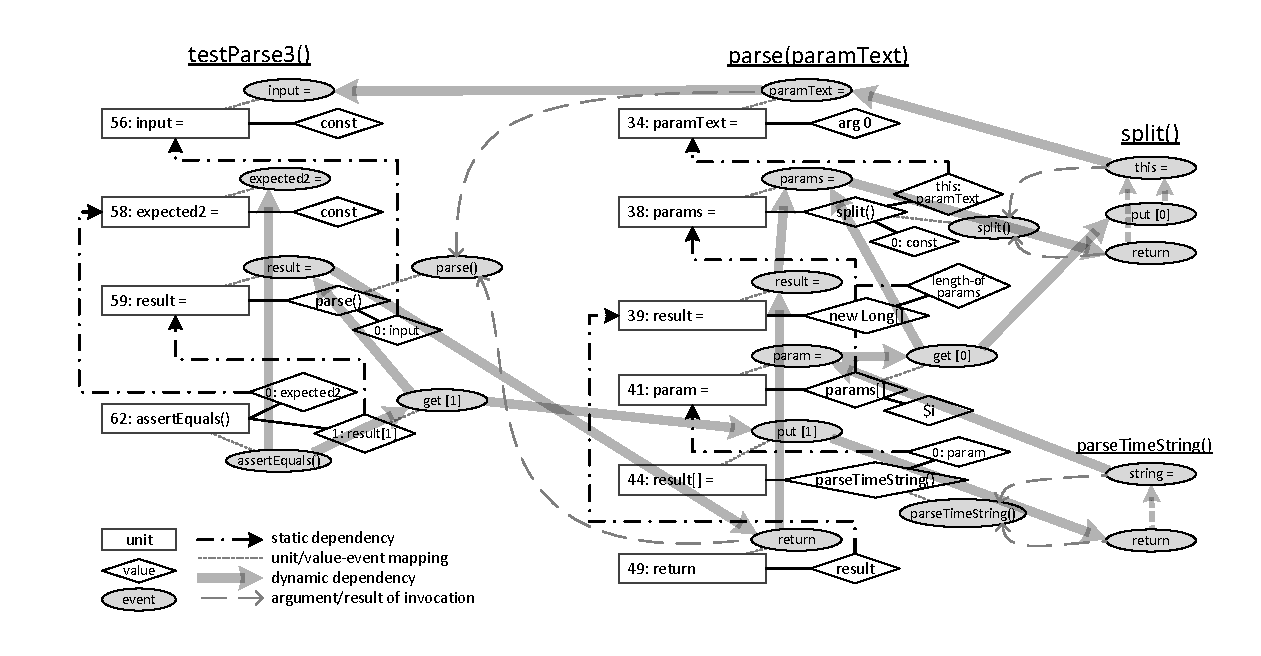
\includegraphics[width=\linewidth, clip, trim=12mm 7mm 8mm 7mm]{img/graph}
%\caption{A dynamic dependency graph of trace events, on top of static dependency graphs derived with Soot. For brevity, not all Soot units are shown, the boxing of long values has been omitted, and ``split'' and ``parseTimeString'' are summarized.}
%\label{fig:graph}
%\end{figure*}

\subsection{Computing the Program Dependence Graph}

Our algorithm for computing \acp{pdg} distinguishes between three dependency types: data, control, and choice dependencies.
The first two types have been used by many authors since the original slicing algorithm by Weiser~\cite{weiser81:program_slicing}.

Data dependencies represent the data flow in a program and occur whenever the value of an instruction is the result of a previous instruction.
For instance, the value of ´words´ in \linerefn{lst:countLetters}{5} of ´countLetters´ depends on the result of ´split´. %data-data-dependency korel90

Control dependencies model the control flow and point to instructions that determine whether a statement can be reached during the execution.
The assignment in \linerefn{lst:countLetters}{8}, for instance, has a control dependency to the conditional expression of the for-loop in \linerefn{lst:parse}{7}.
%test-control-dependency korel90

Choice dependencies occur when a statement has multiple possible data dependencies.
In the statement "´var = conditional ? value1 : value2´", the value of ´var´ depends on either ´value1´ or ´value2´, but never both.
Even though ´conditional´ does not directly affect the value, it determines which of the two options is used; thus, it is a choice dependency.
More formally, choice dependencies are control dependencies of data dependency candidates that are not also control dependencies of all other candidates.
Unlike the other two dependency types, choice dependencies are not simple edges in the graph, but rather tree-like structures that combine it with other dependency edges.
\Cref{lst:choiceExample} shows an example of a nested choice dependency.
Variable ´x´ in \linerefn{lst:choiceExample}{9} has three value dependency candidates, shown with solid red arrows. 
The choice dependencies, shown as dashed blue arrows, link to the conditional expressions that determine the choice.
The tree structure models the relation between the five dependencies.

It should be noted that choice dependencies are redundant for the purpose of computing accurate slices, which is why they were never considered in related literature.
However, as we will discuss in more detail in \todo{reference}, including this dependency type allows us to create slices closer to a developer's needs.

\begin{lstlisting}[float,caption={Example of a nested choice dependency.},stepnumber=2,numberfirstline=false,label=lst:choiceExample,language=Java]
  /*@\hspace{7mm}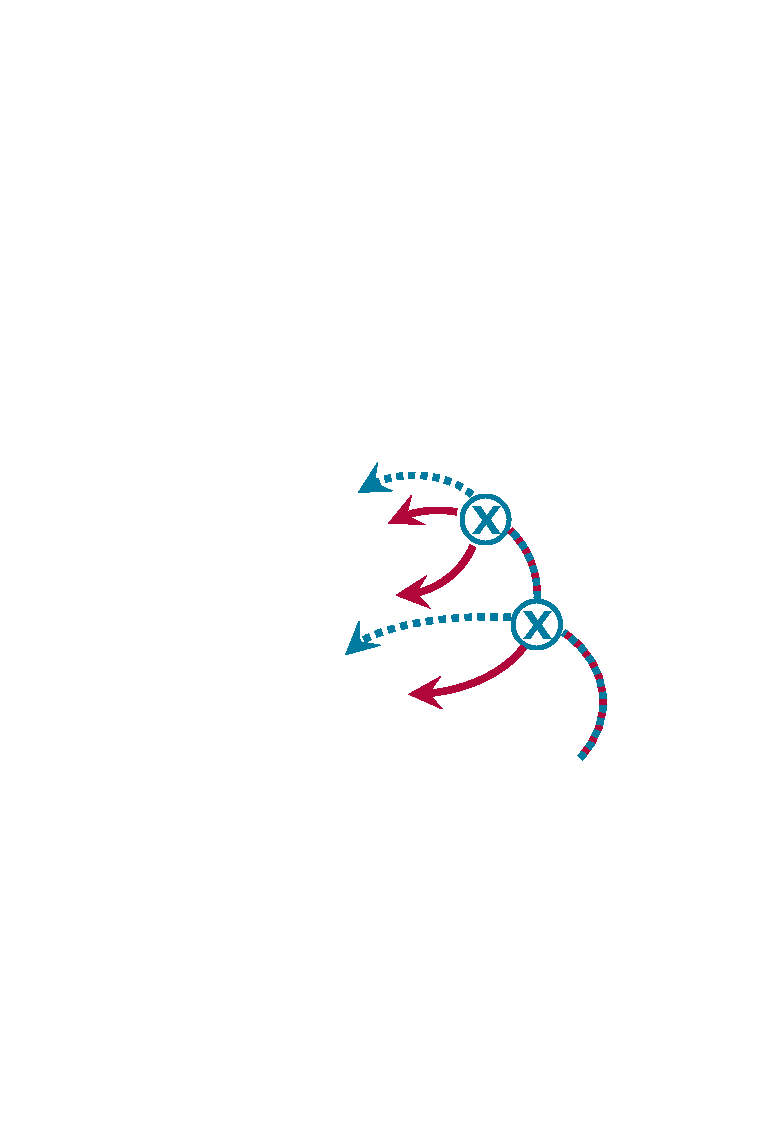
\includegraphics[width=34mm, trim=0mm 45mm 0mm 7mm]{img/choiceexample.pdf}\hspace{-41mm}@*/if (a) {
	  x = 1;
	} else {
	  x = 2;
	} 
	if (b) {
	  x += 2;
	} 
	System.out.println(x);
\end{lstlisting}

The algorithm to build the method-level \acp{pdg} was implemented in Soot, using a \emph{forward flow analysis}~\cite{lam11:the_soot_framework}.
The analysis algorithm has two major operations, the visit and the merge.

In Soot, a method is represented by three-address-code instructions, called "units".
A flow analysis "flows through" (i.e., visits) every unit in a method and allows to pass state in a "flow set" from one instruction to the next.
In our case, the flow set is the \ac{pdg}, as it was computed so far, plus some additional index structures.
The visit operation consists of two steps, as is outlined in \cref{lst:visit}.
First, it collects the dependencies for referenced values, 
then, it creates a node representing the current instruction and adds it to the \ac{pdg}, accordingly to its type.

%\begin{algorithm}
%\caption{The algorithm of the visit operation.}
%\label{lst:visit}
%\begin{lstlisting}[firstnumber=1,stepnumber=5,gobble=0,language=algorithm,tabsize=2]
\begin{lstlisting}[firstnumber=1,float,caption={The algorithm of the visit operation.},stepnumber=5,label=lst:visit,gobble=0,language=algorithm,tabsize=2]
function visit(pdg, unit)
	result := 'copy of' pdg
	dependencies := dependencies_of_values(unit.use_boxes, result)
	if unit 'is a conditional statement' then
	  d := new ControlDependencyNode(dependencies)
		result.control_dependencies.push(d)
	else
	  d := new DependencyNode(unit, dependencies, result.control_dependencies.peek())
		result.store_dependency(unit, d)
		if unit 'is an assignment' then
			result.index_assignment(unit.left, unit)
			if unit.left 'is a variable' then
				result.set_variable_node(unit.left.name, d)
		else if unit 'is a return statement' then
			result.index_return(unit)
		else if unit 'is a throw statement' then
			result.index_throw(unit)
	return result

function dependencies_of_values(values, pdg)
	dependencies := {}
	for each v \in values do
		dependencies << dependency_of_value(v, pdg)
	return dependencies

function dependency_of_value(value, pdg)
	if value 'is a local variable' then
		return pdg.get_variable_node(value.name)
	else if value 'is a method invocation' then
	  pdg.index_invocation(value)
		return new MethodInvocationNode(value.method, 
				dependency_of_value(value.instance, out), 
				dependencies_of_values(value.arguments, out))
	else if value 'is a field reference' then
		return new FieldReferenceNode(v.name, dependency_of_value(v.instance))
	else 
		'handle other value types...'
\end{lstlisting}
%\end{algorithm}

For each unit that is visited, its dependencies are determined from its "use boxes", the values accessed by the unit (cf.~\linesrefn{lst:visit}{3, 20-38}).
\tmpStart
To obtain a list of dependencies from a list of value boxes, each value is examined independently.
If it refers to a variable, the node currently associated with that variable is used.
Field and array accesses are not investigated any further, but a placeholder node is created instead.
Method invocations are also treated as opaque, and no dependency between the invocation result and its arguments is created.
Instead, the dependencies for each argument are determined separately and directly added to the index, with a unique key being created for each argument.
It is expected that the subsequent analysis of the invoked method reveals, if necessary, if and how an invocation's result depends on its arguments.
\tmpEnd

If the unit represents a conditional statement, the dependencies are pushed to the control dependency stack.
Otherwise, they are data dependencies of the unit.
If the unit assigns a variable, it is also registered to be the last unit that changed that variable.
Furthermore, each unit is indexed (cf.~\linesrefn{lst:visit}{10-17, 30}).
The index is stored as a map and will be used later to find the units for recorded events.

The result of the visit step is passed as input to the next unit's visit operation.
If a unit has more than one following unit, (e.g., if it is a conditional jump) a copy of the flow set is passed to each.

When control flow merges, e.g., after a conditional branch closes, two or more flow sets have to merge into one, which can then be passed to the next unit.
Thus, the second major operation of our algorithm is the merge. 
In the merge step of the analysis, the result is a copy of the first incoming flow set, which is then merged with the second incoming set, as outlined in \cref{lst:merge}.

\begin{lstlisting}[firstnumber=1,float,caption={The algorithm of the merge operation.},stepnumber=5,label=lst:merge,gobble=0,language=algorithm,tabsize=2]
function merge(in1, in2)
	result := 'copy of' in1
	if in2.control_dependencies != result.control_dependencies then
	  choice_dependencies := 'disjunctive union' in2.control_dependencies \delta result.control_dependencies
		result.control_dependencies.remove(choice_dependencies)
	else
	  choice_dependencies := {result.control_dependency_stack.pop()}
	for each var \in in2.variable_nodes do
		result_value := result.get_variable_node(var.name)
		if var.value != result_value then
      merged_value := new ChoiceDependencyNode(
            choice_dependencies, var.value, result_value)
			result.set_variable_node(var.name, merged_value)
	return result
\end{lstlisting}

To merge two flow sets, first their control dependency stacks have to be aligned.
If the stacks contain different elements, only dependencies from both stacks are kept.
If both stacks are identical, for instance when merging the then- and else-branch of an if-statement, the topmost element of the stack is removed.

Then, all variables that have different values have to be merged.
Instead of a definite unit, the new value is a choice of the two previous values, indicating that in the dynamic slice only one of the options will actually apply.
Thus, the control dependencies that have been removed during the merge are added here as choice dependencies.

By visiting all instructions in a method and merging the intermediate \acp{pdg} of all possible execution paths, the algorithm eventually produces a complete method-level \ac{pdg}.
For reference, \cref{fig:graph_static} shows the data dependencies of the \acp{pdg} of ´countLetters´ and ´testCountLetters´.

\begin{figure*}[t]
\centering
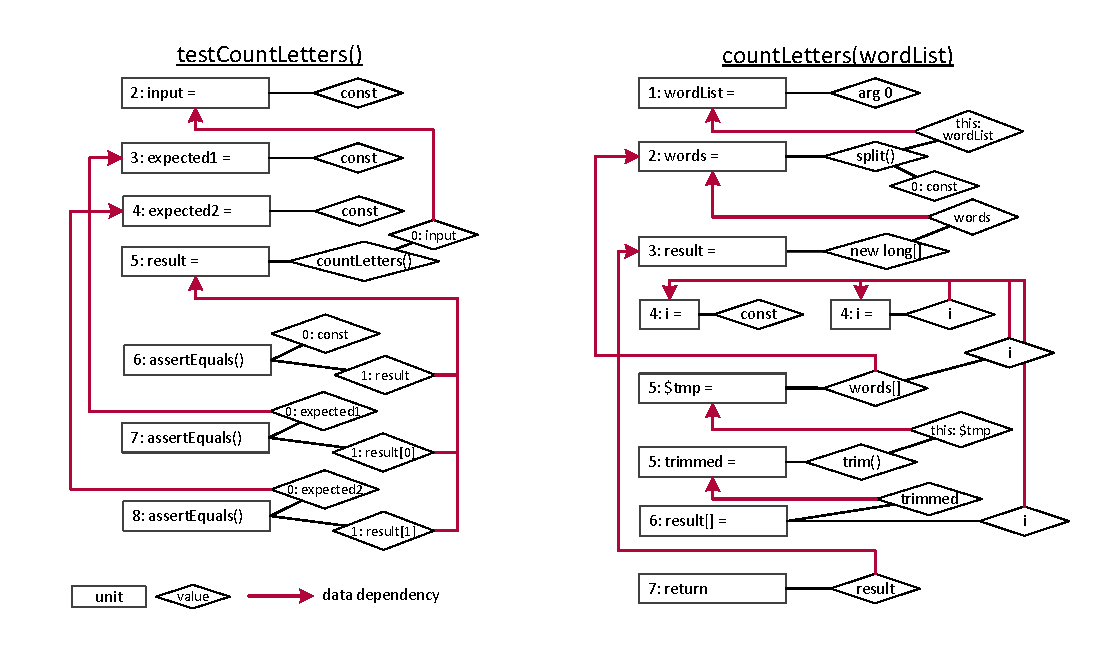
\includegraphics[width=.90\linewidth, clip, trim=12mm 7mm 7mm 7mm]{img/graph_static}
\caption{Data dependencies in the method-level \aclp{pdg} of \lstinline+countLetters+ and \lstinline+testCountLetters+.}
\label{fig:graph_static}
\end{figure*}

\subsection{Building the Dynamic Dependence Graph and Slice}



%Previous "accurate" dynamic slicing algorithms based on \acp{ddg} work by first building a complete \ac{ddg} and then deriving the slice as a subgraph~\cite{agrawal_90_dynamic_program_slicing,zhang_03_precise_dynamic_slicing_algorithms, wang_08_dynamic_slicing_on_java}.
%Our algorithm builds the \ac{ddg} and the slice together, constructing only as much of the \ac{ddg} as is needed to compute the slice.
%Since the method-level \acp{pdg} that form the foundation for the \ac{ddg} are also computed on demand only, our algorithm can potentially save a lot of unnecessary work.

The \acf{ddg} is built by combining the \acfp{pdg} with an execution trace.
In the \ac{ddg}, every node is an event, a recorded execution of an instruction.
Possible events are field and array accesses, variable assignments, and statements with non-local control flow, \ie, method calls, method returns, and exception throws and catches.

The basic structure of the algorithm for building the initial slice is summarized in \cref{lst:slicealgo}.
Initially, the slice is an empty set and the slicing criteria are a set of selected events.
Each event carries flags signifying which types of its dependencies are to be included in the slice.
For events that are not slicing criteria, these flags are not initialized yet.
To begin the slicing, the criteria events are, one by one, added to the slice.

\begin{lstlisting}[float=t,language=algorithm,label=lst:slicealgo,caption={Simplified algorithm for building the slice}]
	function build_slice(criteria)
		slice := {}
		for each event \in criteria do
			''asynchronous:'' add_to_slice(slice, event)
		return slice
		
	function add_to_slice(slice, event)
	  if ~event.has_unresolved_dependencies then return
		slice << event
		pdg := event.method.program_dependence_graph
		static_dependencies := pdg.get(event.instruction, event.dependency_flags)
		for each dependency_link \in static_dependencies do
			for each prev_event \in last_previous_events(event, dependency_link) do
			  prev_event.inherit_dependency_flags(event)
				''asynchronous:'' add_to_slice(slice, prev_event)
\end{lstlisting}

For every event being added to the slice, it is first checked if it has any unresolved dependencies.
This prevents negative slicing criteria, events with every dependency type disabled, from being added to the slice and other events from being processed multiple times.
If the event has unresolved dependencies, it is added to the result set. 
Then its dependencies are resolved.

To find an event's dependencies, first its method-level \ac{pdg} is obtained.
%The graph is computed using the algorit
Every event is associated with an instruction.
Looking up the instruction in the \ac{pdg}, while considering the event's dependency flags, reveals the static dependencies.
For each static dependency, the set of latest matching events is looked up in the execution trace.
Each event then inherits the dependency flags, unless it is a criteria event for which the flags are fixed, and is added to the slice recursively.

Finding the latest matching events can be simple in the case of linear computation steps, but can also involve several intermediate steps.
For example, \cref{fig:graph_dynamic_arg} shows how dependencies of a method call argument are resolved.
The \ac{pdg} of ´assertEquals´ shows that the variable ´expected´ is initialized with the first argument of a method invocation.
Using the execution trace, the variable event can be linked to a method call of ´assertEquals´ call in \linerefn{lst:testCountLetters}{8} of ´testCountLetters´.
The \ac{pdg} of ´testCountLetters´ shows that the first argument has a data dependency to the assignment of variable ´expected1´, for which then the corresponding event is selected from the trace.
A data dependency is now created between the two events and the slicing continues.

\begin{figure*}[tp]
\centering
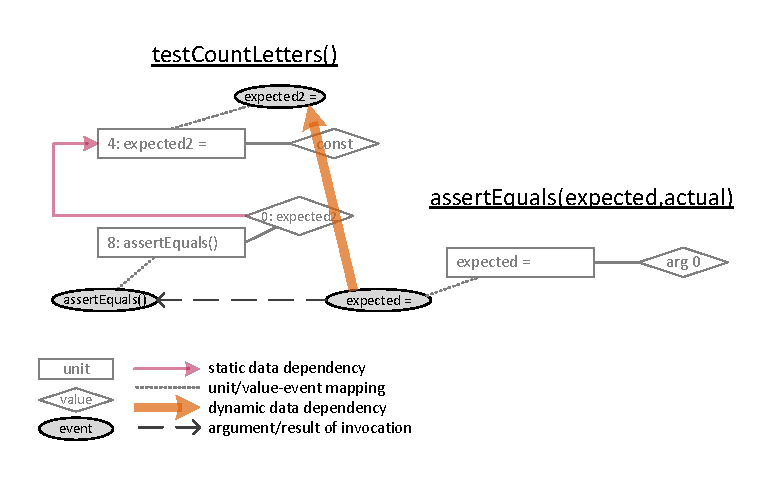
\includegraphics[width=.8\linewidth, clip, trim=6mm 6mm 6mm 7mm]{img/graph_dynamic_arg}
\caption{A data dependency edge between a method invocation argument and a variable.}
\label{fig:graph_dynamic_arg}
\end{figure*}

Likewise, for ´actual´, the second parameter, a dependency can be traced to reading the second element in the ´result´ array.
From here, two data dependencies can be found, as \cref{fig:graph_dynamic_array} shows.
The first concerns the identity of the array object and is resolved using the \ac{pdg}, which points to the assignment of the ´result´ variable.
The second dependency concerns the value of the second element, which was assigned in a different method and can therefore not be tracked using the method-level \ac{pdg}.
However, scanning the execution trace reveals that the element was assigned by an event in line 6 of ´countLetters´.

\begin{figure*}[tp]
\centering
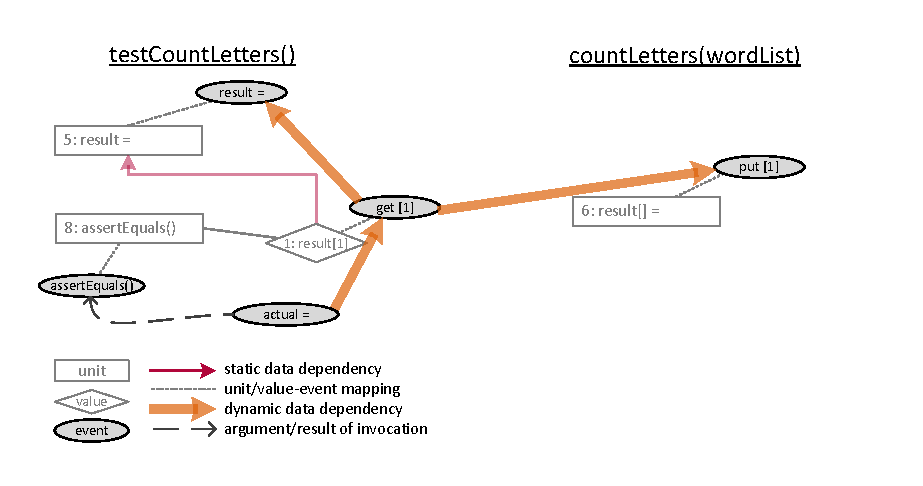
\includegraphics[width=.8\linewidth, clip, trim=6mm 7mm 19mm 7mm]{img/graph_dynamic_array}
\caption{Dependencies of an array-read event, one is resolved using the method-level \aclp{pdg}, the other using the execution trace.}
\label{fig:graph_dynamic_array}
\end{figure*}

As was mentioned before, when one method calls another, the \ac{pdg} of the first method contains no dependency links between the call's return value and its arguments.
Instead, a dynamic data dependency is created between the event receiving the value in the first method and the return event of the second.
As shown in \cref{fig:graph_dynamic_method}, further analysis of the second method will then reveal if there is a dependency chain leading to the argument values.
The invocation event itself is not a data dependency to any event, as it has no side effects, but is a control dependency to the events in the called method.

\begin{figure*}[tp]
\centering
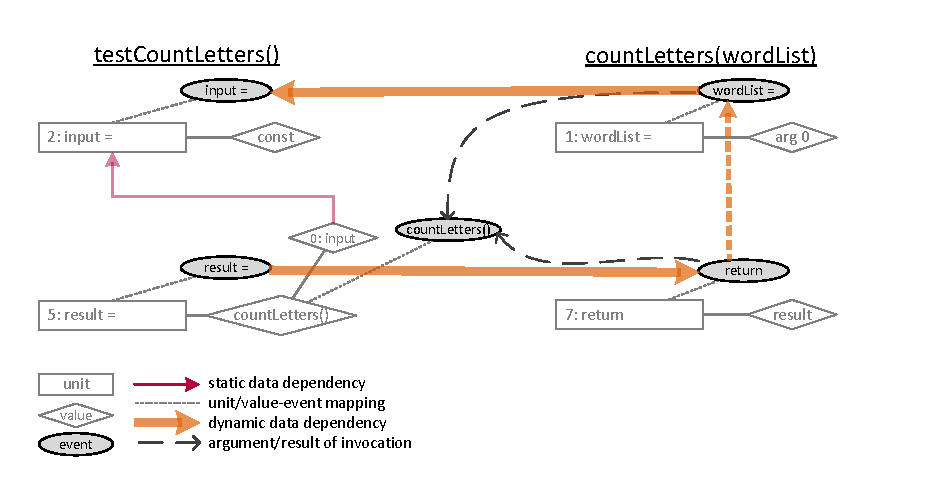
\includegraphics[width=.8\linewidth, clip, trim=6mm 7mm 16mm 7mm]{img/graph_dynamic_method}
\caption{A method call result transitively depends on the method call arguments if and only if analysis of the method reveals such a relation.}
\label{fig:graph_dynamic_method}
\end{figure*}

As events are resolved and successively added to the result set, the slice is eventually completed.
\Cref{fig:graph_dynamic} shows the data dependencies of the \ac{ddg} for a slice on the arguments of the call in line 8 of ´testCountLetters´.

\begin{figure*}[tp]
\centering
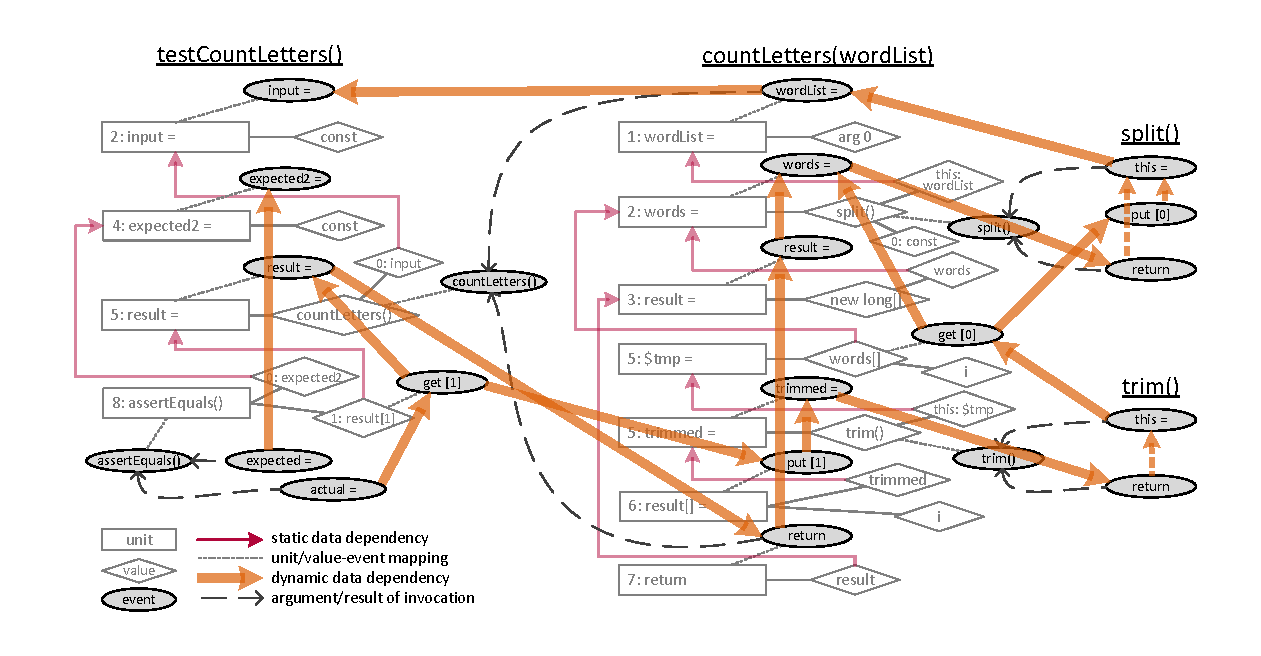
\includegraphics[width=\linewidth, clip, trim=11mm 7mm 8mm 7mm]{img/graph_dynamic2}
\caption{A partial dynamic dependency graph of trace events, on top of static dependency graphs derived with Soot. For brevity, not all Soot units are shown, events related to the loop-variable "i" are omitted, and "split" and "trim" are summarized.}
\label{fig:graph_dynamic}
\end{figure*}

%Because our algorithm does not require the execution trace to be read sequentially, the processing of events can be parallelized, increasing the throughput of our approach.

\subsection{Incremental Slice Configuration}

\tmpStart

As indicated in the \cref{lst:slicealgo}, the algorithm is designed to follow all dependency links concurrently.
This allows using parallelization to improve the performance of the slicer.
The amount of concurrency is only limited by the theoretical maximal level of concurrency in the original program.
This is to be expected as the slicer is, in some sense, just evaluating the program backwards.

However, we also let the slicing run concurrently to the user interface.
Twice per second, we update the different debugging views, such as variable and trace explorer, to use the latest intermediate result.
This way, we not only don't have to freeze the user interface, but we can allow developers to continue working even if the computation the whole slice has not finished yet.
Developers can even change the slicing criteria while the slicer is still running.

Adding another event to the slicing criteria works similarly to building a new slice, the major difference being that the slice is not initially empty.
Changing the dependency type of an event, e.g., from data to control, is a combination of removing an event and adding it again with different flags.

When developers want to remove an event from the slice, we need to know when to cascade the removal to its dependencies.
As the dynamic dependency graph is acyclic, we can use reference counting for this.
However, we need to independently count the references for each dependency type.
When the counter for one of the dependency types reaches zero, dependencies of that type are unlinked recursively.

\tmpEnd


%Before the dependencies of an event can be found, it has to be mapped to a Soot unit.
%The event provides class and method name, line number, and byte-code index as locational information.

%Alas, we were not able to find the corresponding unit based on the byte-code index.
%Instead, the event type and line number are used to look-up units in the index that was created during the flow analysis.
%For an averagely structured Java program, ambiguities occur only rarely.
%As shown on the bottom left of \autoref{fig:graph}, in our example the slice would begin with the \verb+assertEquals+ invocation, which can be mapped to the invocation unit in \linerefn{lst:test}{62}.

%Once the unit has been identified, its dependencies are looked-up and converted back to events.
%Reachability dependencies are included only if they have been explicitly requested.
%%How events are looked-up depends on the type of the dependencies.
%The dependency value's line number and the current event's step number are used to identify the most recent matching event.
%However, the strategy of the look-up also depends on the type of the dependency value.

%If the dependency is an assignment statement of a variable, the last variable change event in that line is looked-up.
%For instance, the dependency between the \verb+assertEquals+ invocation and the \verb+expected2+ assignment is created this way.
%If it is a choice of multiple variable assignments, each assignment is looked-up and, if more than one is found, only the most recent will be used.

%For field and array value dependencies, first the according get-event is looked-up.
%Then, the last set-event before the get is found.
%For instance, this allows us to create a dynamic dependency between \verb+assertEquals+ and the array assignment in the second iteration of \verb+parse+ (shown on the right-hand side of \autoref{fig:graph} as the ``put'' event linked to the assignment in \linerefn{lst:parse}{44}).
%Finding the get as an intermediate step is necessary to avoid situations where the field has been changed between access and usage, e.g., as in \verb/int id = counter++/.

%If the value stems from an argument, first the calling method is determined from the trace data. 
%Then, the argument is looked up in the index of the dependency graph of the calling method.
%Finally, the dependencies retrieved this way are resolved recursively.
%To get the result of an invocation, the method call event is looked-up and its respective return event is found.
%As \autoref{fig:graph} shows, the invocation of \verb+parse+ is not part of the dynamic dependency graph because it is an event without side effects.
%However, it serves as the link to create dependencies between events of the two methods.

%All events that are found this way are added to the slice.
%If an event was found via a unit, this information is retained and reused when computing the dependencies for that event.

%The final list of events is the used by the debugger to visualize the program flow and to skip unrelated events during stepping.

%In principle, the Slice Navigator can run on top of any slicing algorithm.
%However, for most effectiveness, the algorithm should satisfy three criteria:
%First, it should be able to quickly produce useful intermediate results to avoid interrupting developers in their work.
%Second, if it distinguishes between different types of dependencies, the differences between those types should be easily understandable for developers.
%This way, additional helpful information can be communicated to the user and better customization of the slice is possible.
%Finally, it should support incrementally changing the slicing criteria.
%The algorithm we use in our prototype is specifically engineered to meet these criteria.

%The algorithm we use in our prototype is based on previous work~\cite{treffer_dynamic_2014} and specifically engineered to meet these criteria.
%When building the dependency graph between instructions, the algorithm distinguishes between three types of dependencies.
%
%\emph{Value dependencies} occur when the the value of an instruction is derived from another instruction's value.
%In the slice navigator, they are represented with a red equality sign.
%
%Instructions that determine if another instruction can be reached are \emph{reachability dependencies}, indicated by a yellow arrow.
%Typically, these are method invocations and instruction in conditional statements.
%
%Sometimes, a value depends on only one of multiple candidate values. 
%A \emph{control dependency} determines which of these candidates is used.
%More formally, control dependencies are reachability dependencies of value candidates that are not also reachability dependencies of all other candidates.
%In the navigator, they are indicated by a blue~"X".
%
%Developers can now combine these different dependency types to adjust the slice for specific purposes.
%Clicking on an event's dependency symbol brings up a dialog that allows to choose which dependencies of that event to include.
%This way developers can, for instance, put a focus on how a value was computed or how an instruction was reached.
%It is also possible to remove all dependencies of an event, for instance if it is known to be correct and its history is not of interest, thereby moving the focus of the slice to less well-understood parts of the program.


%Typically, static and dynamic slicing algorithms focus on finding statements belonging to a slice.
%However, in many cases statements are executed multiple times in a single program run and not all executions are relevant for the slice.
%Therefore, our algorithm focuses on state-changing events, i.e., actual executions of statements, instead of the statements themselves.

%On the highest level, our algorithm to compute a dynamic slice works as follows:
%The output of the algorithm will be a sorted set of events.
%The target event, i.e., the event for which the slice was requested, is added to both the result set and a queue of unprocessed events.
%Then, until the queue is empty, an event is polled and its dependency events are determined as follows:

%%Firstly, the event is mapped to a unit of a \verb+SootMethod+.
%Firstly, the event is mapped to a statement in the code.
%Secondly, Soot is used to obtain a static dependency graph for that method (the graph is cached for reuse).
%Thirdly, the statement is looked-up in the graph and candidate dependency statements are mapped back to events.

%Each dependency event that is not yet part of the result set is added to both the result and the queue.
%Finally, the result set is returned.
%\tmpEnd

\section{Interactive Dynamic Slicing: a new Debugging Workflow}
\label{sec:workflow}

We presented an efficient configurable dynamic slicing algorithm that can produce different slices depending on developer's needs.
The support for frequent and quick reconfigurations not only allows developers to change the slice as they debug the code, it also alleviates them from having to get the entire configuration right on the first try.
However, for a slice to be really useful to developers, it has to be debuggable.
Because our algorithm does not produce executable slices, slicing support has to be directly integrated in the debugger.

\Acfp{odb} are debuggers that not only allow developers to move forwards and backwards through a program execution, but can instantly access any point in time~\cite{lewis03:debugging_backwards_in_time}.
A common way of implementing \acp{odb} is the post-mortem approach: the execution of a program is first recorded and then a debug session is simulated by replaying the execution trace~\cite{lewis03:debugging_backwards_in_time, pothier07:scalable_omniscient_debugging}.

Both omniscient debugging and (dynamic) slicing changed the way how developers approach fault localization.
Combining omniscient debugging and and dynamic slicing in one tool, we found synergies between both approaches that enable developers to follow a new debugging workflow.

\tmpStart

In this section, we present \emph{interactive dynamic slicing}, a new debugging workflow that combines omniscient debugging and dynamic slicing. 
While developers omnisciently debug a dynamic slice, at any point they can add or adjust slicing criteria. 
Changes are applied instantly, without interrupting the debug session. 
%A new UI component, the Slice Navigator, provides a unique view on the program’s execution by combining relevant information from both the ODB and the slicing subsystem.
A new UI component, the Slice Navigator, enriches the debugging experience in multiple ways by combining access to both the \ac{odb} and the slicing subsystem.
%We present the Slice Navigator, a UI component that combines back-in-time
%debugging with a complementary tool, a dynamic slicer, to enrich the debugging
%experience in multiple ways. 
Firstly, the Slice Navigator supports developers’ short term memory
by providing a summary of relevant program state and context for the current
instruction. Secondly, it provides an alternative to breakpoints as it can be used
to control the debugger to jump to related instructions, such as the last change of
a variable. Thirdly, it allows to directly reconfigure the slicing criteria, enabling
developers to minimize the search space of active code without interrupting the
debugging workflow.
With the Slice Navigator, developers isolate a bug by iteratively slicing away correct code, homing in on the problem. 
This reduces interruptions in developer flow by minimizing context switches between tools and shortens waiting time as already recorded run-time data can be re-used.

%We also describe the user interface of the Slice Navigator, how it presents information about the slice, and how it can be used to control the debugger.
\tmpEnd
\tmpStart

\subsection{Getting Started}
\label{sec:example}

Very often, the starting point for a debug session is a reproducible observable program failure, preferably in the form of a failing unit test.
Using an omniscient debugger, developers halt the execution at the failing line of code to observe the program state.
From here, they want to backtrack the erroneous state.
However, they quickly realize that the code contains many other side effects making it hard to follow the state of interest.

Using a pure omniscient debugger, developers would now have to track the relation of states to identify the infection chain. 
In other words, they have to manually create a dynamic dependence graph using only their short-term memory. 
When slicing features are supported, they might rather leave that task to the tools.
\tmpEnd
With slicing integrated in the debugger, developers can choose to slice on erroneous state in the debugger's variables view.
This will set the variable or field as a slicing criterion and start the slice computation.
\tmpStart
%The initial code analysis can take a few seconds.
%The performance of our prototype implementation is evaluated in \todo{section ?} .
%Once the slice is computed, all debugging views, such as the trace and the variable view, will show instructions or variables not belonging to the slice only in gray.
%Stepping through the execution will skip instructions not belonging to the slice.

In the remainder of this section, we use a small code example to demonstrate how we integrated existing and new tools into an improved debugging workflow,
and to explain the user interface and internals of the Slice Navigator. 
\Cref{lst:example} shows two Java classes and a failing JUnit test case.
In our scenario, after noticing a failed test case, the developer chooses to slice on the arguments of the ´assertEquals´ invocation in \linerefn{lst:example}{31}.
Because we are using only a minimal example, the resulting slice contains almost the entire program.
When we tested the Slice Navigator on real open source programs, this step often already removed a lot of code.
%\tmpEnd
%\Cref{fig:calltree} shows the first two levels of a call tree from a test in the Drools framework.
%Slicing on one of the tests assert statements removed many events, which are shown in gray, from the execution.
%\tmpStart
%
%\begin{figure}
%\centering
%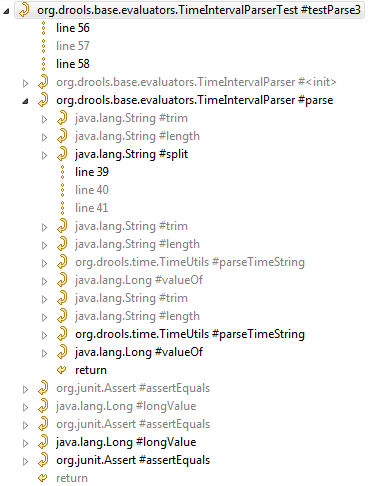
\includegraphics[width=.5\linewidth]{img/calltree}
%\caption{A tree of method invocations. Gray nodes are not part of the current slice.}
%\label{fig:calltree}
%\end{figure}

\begin{lstlisting}[float=t,label=lst:example,caption={Example program with a failing test case},language=Java]
	class Square implements Shape2D {
			private double length;
			public Square(double length) { 
					this.length = length;
			}
			
			@Override
			public double getArea() { 
					return length * length;
			}
	}
		
	class Pyramid implements Shape3D {
			private Shape2D base;
			private double height;
			public Pyramid(Shape2D baseShape, double height) {
					base = baseShape;
					height = height;
			}
			
			@Override
			public double getVolume() { 
					return base.getArea() * height / 3; 
			}
	}
	
	class PyramidTest {
			@Test
			public void test_getVolume() {
					Shape3D shape = new Pyramid(new Square(2), 6);
					assertEquals(8, shape.getVolume());
			}
	}
\end{lstlisting}

Nevertheless, for a complex program the initial slice can still be too large to allow an efficient search for the problem.
In this case, the developer can now use the Slice Navigator to get an overview of the execution and to iteratively adjust the slicing criteria.

\subsection{The Slice Navigator}

\begin{figure}
  % picture on first page :)
	\centering
		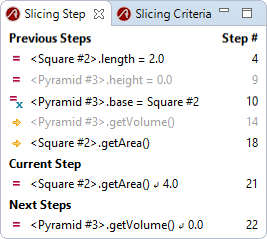
\includegraphics[width=0.40\linewidth]{img/slice1.png}
	\caption{The Slice Navigator shows context for the current debug step. Steps directly related to the current step are listed in black, steps with overarching dependencies in gray. Small icons indicate how the steps are related.}
	\label{fig:slice1}
\end{figure}

To produce a slice, dynamic or static, slicing tools have to build up deep knowledge of a program's internal workings.
In the end, only a binary mapping about which instruction to include or exclude from the program is returned, and most of the slicer's internal knowledge is discarded.
Hence, the initial motivation for the Slice Navigator was to make better use of a slicer's internal data.
However, since  dependency graphs are typically too vast to be visualized at once, we propose to use that data to guide developers while they debug the slice.

The first purpose of the Slice Navigator is to aid the developer's short-term memory.
It provides a quick overview over previous and upcoming events, and how they relate to the current instruction.
\Cref{fig:slice1} shows a screenshot of the Slice Navigator with the execution of the example test-case halted on the ´return´ instruction of ´getArea()´ in \linerefn{lst:example}{7}.

A step, or event, is any instruction that has a side effect on the program state.
"Previous Steps" lists all past events that the current or any future events depend on.
Likewise, "Next Steps" shows all events that depend on the current or a previous event.
%
If a step is shown in black, it has a direct dependency link to the current step.
Steps shown in gray have dependencies that go beyond the current step.
I.e., gray "previous steps" have dependency links to "next steps", and vice versa.


%\subsection{Filling the Slice Navigator}

To fill the Slice Navigator, we iterate over the events in the slice, ordered by step number, beginning at the current step, and collect the events to be shown.
Events directly related to the current step will be flagged as such, so that they can be highlighted.

Events at the current step and their dependencies are always collected.
For events in the future, it is first determined if they have direct dependencies that are in the past.
If such dependencies exist, they are collected together with their respective future event.

However, our collection algorithm considers two special cases:
First, reachability dependencies are not collected except for the current step.
This measure is taken to prevent the entire method stack from appearing in "previous steps" and all future variable changes in "next steps".
The second special case are transparent classes.
Classes of the JDK are flagged as transparent, and all their internal events, i.e., all events except direct accesses from non-transparent classes, are resolved immediately and never appear in the navigator.
% /Filling the SN

Simply by looking at the previous and next steps, the developer can understand at a glace how the current instruction fits into the greater scheme.
This is particularly useful if the current instruction was reached via a breakpoint, in which case it is not always obvious at which point in time it was hit.

To obtain this kind of information with a regular debugger, developers need to analyze the execution stack and maybe even inspect lower stack frames.
But even then it is not always obvious which part of the program state that is still reachable is actually used again.
Unlike a typical debugger's variable view, the Slice Navigator only shows relevant variables, and also shows relevant object fields on the first level.

Further, the Slice Navigator shows details about the dependency graph that was used to compute the current slice.
Small icons indicate how the events of the slice are related.
A red equal sign indicates data dependencies, a yellow arrow control dependencies, and a blue X choice dependencies.

The second purpose is to serve as a convenient interface to the debugger.
Debugging with the Slice Navigator is simple:
To investigate the origin of a value, developers can simply click on it to move the execution to that point in time.
This way, the slice navigator allows to efficiently follow infection chains of erroneous state.
Likewise, it is easy to follow up on the impact of an instruction by navigating to its future dependencies.

As developers continue to debug, their understanding of the program and their questions change.
The slice they initially created will at some point no longer fit those questions.

Thus, thirdly, using the Slice Navigator developers can not only control the debugger, they can also adjust the slicing criteria.
Developers can combine different dependency types to adjust the slice for specific purposes.
Clicking on an event's dependency symbol brings up a dialog that allows to choose which dependencies of that event to include.
This way developers can, for instance, put a focus on how a value was computed or why an instruction was reached.
It is also possible to remove all dependencies of an event, for instance if it is known to be correct and its history is not of interest, thereby moving the focus of the slice to less well-understood parts of the program.

\begin{figure}
	\centering
		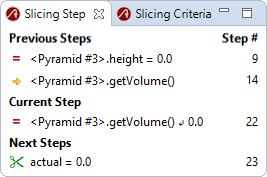
\includegraphics[width=0.40\linewidth]{img/slice2.png}
	\caption{The program halted at \linerefn{lst:example}{21}, after \lstinline{getArea()} was removed from the slice.}
	\label{fig:slice2}
\end{figure}

Whenever a slicing criterion is modified, the slice is updated instantly, without locking the user interface or resetting the current debug session.
In our examples, developers might choose to exclude the result of ´getArea()´ from the slice because  they could determine that it is correct.
As shown in \cref{fig:slice2}, with the computation of the area removed from the slice it is now much easier to see that the wrong result of ´getVolume()´ was caused by a wrong value in the ´height´ field.

As mentioned before, instructions and states not belonging to the slice are still shown in the IDE, mostly to serve as an orientation help, to provide context to the current operations.
However, it might also happen that a value or instruction outside of the slice catches a developers attention.
In this case, they can choose to add it as another slicing criterion and the slice is immediately expanded.
Again, this happens without interrupting the developer's work.

After some preliminary user testing, we added two shortcuts for frequently used operations.
Right-clicking an entry immediately sets it as a negative slicing criterion, removing it entirely from the slice, while double-clicking an entry sets it as a slicing criterion and removes all other criteria.

With the power to quickly modify the slice as needed and with currently relevant dependencies laid out, developers can efficiently reduce the search space for a fault.



\section{Prototype Implementation}
\label{sec:impl}

\todo{reuse the pdg \cite{ottenstein84:the_program_dependence_graph}}

The Slice Navigator is part of a set of debugging tools that we implemented as a plug-in for the Eclipse IDE\footnote{\url{http://eclipse.org}}.
%
%\subsection{Framework}
%
The high-level architecture of our prototype consists of three components: the tracer, the event database, and the omniscient debugger including the slicing module.

%The tracer is implemented as a Java agent that modifies the bytecode of a program to insert tracing instructions that log all events into csv files.
%With our Eclipse plug-in, the developer can initiate an omniscient debug session by selecting a customized launcher in the run configuration.
%The launcher will add VM arguments to the execution to configure the tracer.
%Once the execution completes, the launcher will automatically import the trace data into a previously configured database.
%We provide launchers for basic Java applications and for JUnit test suites.
%For JUnit launches, the tracer will treat each test case as an independent execution and ignore code of the testing framework.
%
%The database stores all events of a set of executions.
%It is possible to set up one database per project or one for the entire workspace.
%We currently support HSQLDB, MySql, and SAP Hana, but in principle any relational database can be used.
%\todo{details on model, ui}
%
%The omniscient debugger consists of a set of Eclipse views that allow to debug a Java application based on the data from the database.
%It is a post-mortem debugger, i.e., it simulates a debug session while the actual program has already terminated.


\subsection{Modeling the Execution Trace}

Debuggers are a special kind of runtime analysis tools.
Basically, there are two ways to implement a runtime analysis.

A live analysis evaluates the program as it is executed; as soon as, or even before, the program terminated, the result of the analysis is available.
Common debuggers typically fall into this category.

A post-mortem analysis first records aspects of the programs execution and then analyses the recorded data.
Sometimes, this approach has the advantage that multiple analyses may be run iteratively, without having to re-execute the program.
This disadvantage of this approach is that, depending on the granularity of the recorded data, it requires much more memory.

Backwards debuggers can be implement with both the live and the post-mortem approach.
In the scenario described above, where the debug session begins at the occurrence of a failure, it does not make much of a difference.
In other use cases, however, the look-ahead that is possible with the post-mortem approach can make the difference between a simple backwards and a fully omniscient debugger.

Many strategies have been proposed to reduce the amount of data that has to be captured to allow a replay of the execution~\cite{pothier07:scalable_omniscient_debugging, lienhard08:practical_object-oriented_back-in-time_debugging}.
However, since we aim for an omniscient approach, we will record almost everything.

Figure \ref{fig:model} shows how the execution trace is modeled.
The trace model consists of two parts.

\afterpage{

\begin{figure}[tp]
\centering
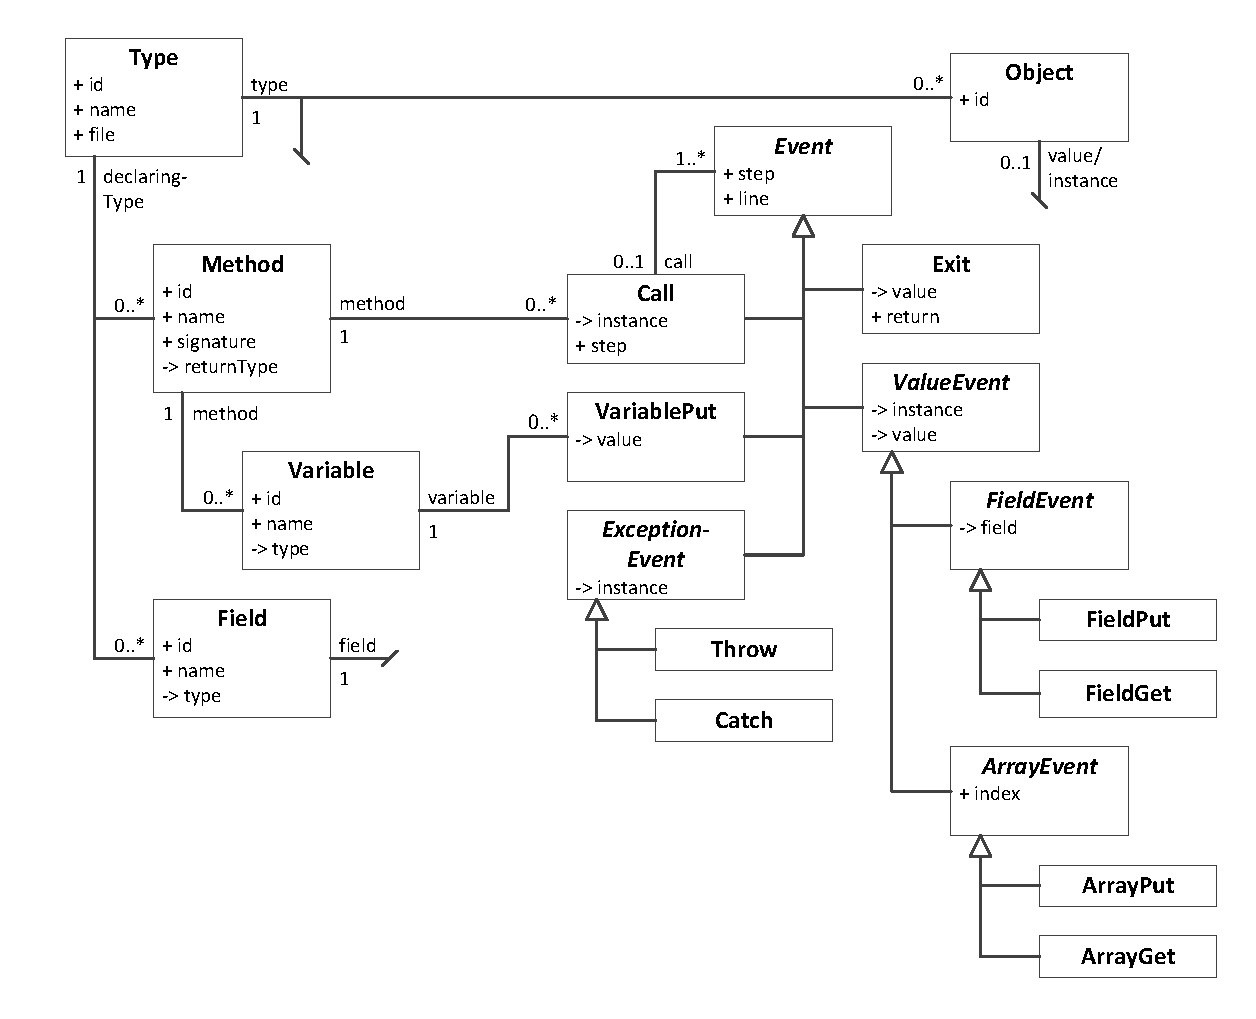
\includegraphics[width=\textwidth, clip, trim=5mm 5mm 5mm 5mm]{img/model.pdf}
\caption{Trace Model}
\label{fig:model}
\end{figure}

\clearpage
}

The static part describes the application's code on a high level.
Classes, fields, methods, and variables are represented with enough properties to find them in the code base, so that they can be referenced from the actual trace data.

The dynamic part identifies all objects that occurred during the execution and contains events that happened with these objects.
Every event is identified and ordered by a step number and contained in a parent method call (except for the root call).

The program flow is described with call events, which reference the method and the instance on which it was called, and their respective exit events which provide the result value and indicate whether the method terminated via return or exception.
Additional program flow is provided by exception throw and catch events.

Value events indicate changes and side-effects of the program state.
Represented are field and array reads and writes, as well as variable changes.
This way, the state of an object or the variable assignments at a certain point in time can be easily derived from the latest respective set events.

To obtain the execution trace, a tracer is injected into the program
The tracer is implemented as a Java agent that modifies the bytecode of a program to insert tracing instructions that log all events into csv files.
With our Eclipse plug-in, the developer can initiate an omniscient debug session by selecting a customized launcher in the run configuration.
The launcher will add VM arguments to the execution to configure the tracer.
Once the execution completes, the launcher will automatically import the trace data into a previously configured database.
We provide launchers for basic Java applications and for JUnit test suites.
For JUnit launches, the tracer will treat each test case as an independent execution and ignore code of the testing framework.

The database stores all events of a set of executions.
It is possible to set up one database per project or one for the entire workspace.
We currently support HSQLDB, MySql, and SAP HANA, but in principle any relational database can be used.
Based on this model, it is possible to develop a debugger that can revert and replay the execution of a program and provide snapshots of the state at any point in time.

\subsection{Omniscient Debugging in Eclipse}

The omniscient debugger consists of a set of Eclipse views that allow to debug a Java application based on the data from the database.
They support default debugger features, such as inspecting state and stepping through the program, as well as some more advanced navigation operations.

A recurring debugging task is to find the origin of a value.
%It seems obvious how a backwards debugger can improve the time required to find the source of an error.
%Restarting the debug session becomes virtually unnecessary.
Using the \ac{odb}, developers can step backwards to its source.
If a method call is stepped over by accident (in either direction), the operation can be easily reverted.
Nevertheless, this may still require stepping (backwards) through large parts of the application.
An omniscient debugger, on the other hand, immediately knows where the value was set.

\begin{figure}[ht]
\centering
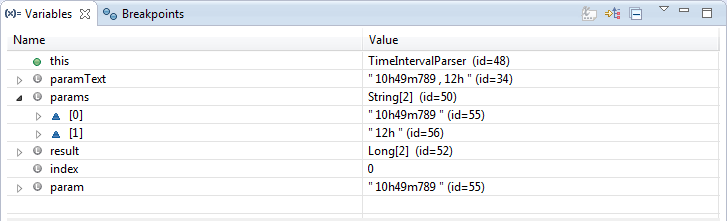
\includegraphics[width=.8\textwidth]{img/variables.png}
\caption{Variables View in Eclipse}
\label{fig:variables}
\end{figure}

Figure \ref{fig:variables} shows the variable view of Eclipse's debugging perspective, which is typically used to spot erroneous values.
With the omniscient debugger extension, developers can directly jump back in time to the assignment of a value simply by double clicking it.
This changes the debugging process as follows:

Developers finds the value and double-clicks to jump to its source.
If they find the value is build from multiple other values, using a formula that seems to be correct, then one of the input values must be erroneous.
To explore the branching dependencies, developers can bookmark the current point-in-time and begin to investigate the first value.
When stepped through the value's creation reveals that it is correct, the bookmark can be used to go \emph{back to the future}.
Developers then use this process to investigate all values until the fault is reached.

As the example shows, another important task is to determine whether a value is valid by examining how it is produced.
Here, the omniscient debugger can assist in multiple ways.
Firstly, instead of showing just the current stack trace, the omniscient debugger can provide a tree of previous and subsequent invocations (cf.~figure~\ref{fig:tree}).
Especially after jumping backwards, the developer may have to regain temporal orientation, where this additional context can be helpful.

\begin{figure}[ht]
\centering
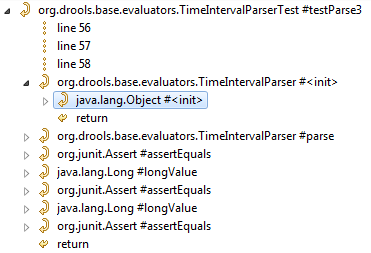
\includegraphics[width=.55\textwidth]{img/tree.png}
\caption{Call Tree}
\label{fig:tree}
\end{figure}

Secondly, the debugger can show the history of a variable, or even an entire object (cf.~figure~\ref{fig:history}).
Mostly, this is helpful when a value is created in a loop or if an object is changed in multiple, different parts of the application over a longer stretch of time.

\begin{figure}[ht]
\centering
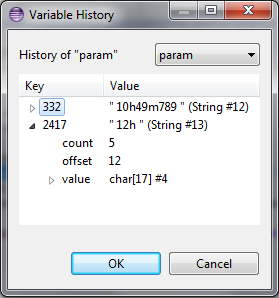
\includegraphics[width=.4\textwidth]{img/history.png}
\caption{Variable History}
\label{fig:history}
\end{figure}

Finally, the debugger knows whether a given value is used again or at all.
By graying out variables and fields that are not accessed again (at least not before their values are changed), the program state that has to be examined by the developer is effectively reduced.

%\subsection{Initial Slice Computation}
%
%In principle, the Slice Navigator can run on top of any slicing algorithm.
%However, to maximize its effectiveness, the algorithm should satisfy three criteria:
%First, it should be able to quickly produce useful results to avoid interrupting developers in their work.
%%Second, it should distinguish between different types of dependencies that are easy to understand and useful for developers.
%Second, it should distinguish between different types of dependencies that provide benefits to developers.
%This way, additional helpful information can be communicated to the user and better customization of the slice is possible.
%Finally, it should support incrementally changing the slicing criteria.
%While it may be acceptable to wait several seconds for the initial slice, slow incremental changes will discourage developers from using slicing to the fullest extent.

%\todo{restructure}
%The algorithm we use in our prototype is based on previous work~\cite{treffer_dynamic_2014} and was specifically engineered to meet these criteria.
%The basic structure of the algorithm for building the initial slice is summarized in \cref{lst:slicealgo}.



\tmpEnd

\section{Evaluation}
\label{sec:eval}

\tmpStart
We evaluated our approach in two ways.
First, we measured the run-time of the slicing component for various operations on a real-world project and found it to be fast enough to be usable in practice.
Second, we let developers locate bugs using different tools and interviewed them about their experience.
The experiment confirmed the usefulness of the Slice Navigator and provided suggestions for further improvements of our tool.
%
%\subsection{Performance Considerations}
%\label{sec:eval}
%
\subsection{Performance Considerations}

One of the main advantages of the Slice Navigator is that it integrates into the debugging workflow.
As such, it is crucial that results are produced in a timely manner, as a waiting time of even a few seconds may interrupt developers in their flow.

To evaluate the performance of our approach on real-world code, we measured the computation of several slices on JUnit tests of an open-source business-process engine\footnote{\url{https://github.com/camunda/camunda-bpm-platform}}.
All tests were run on a 2.0 GHz Intel i7 Processor with 4 cores and and 8 GB RAM, running Windows 8.1.
A MySql database was used to store the trace data.
We repeated every measurement 10 times, all charts show the average values.

\begin{figure}
	\centering
		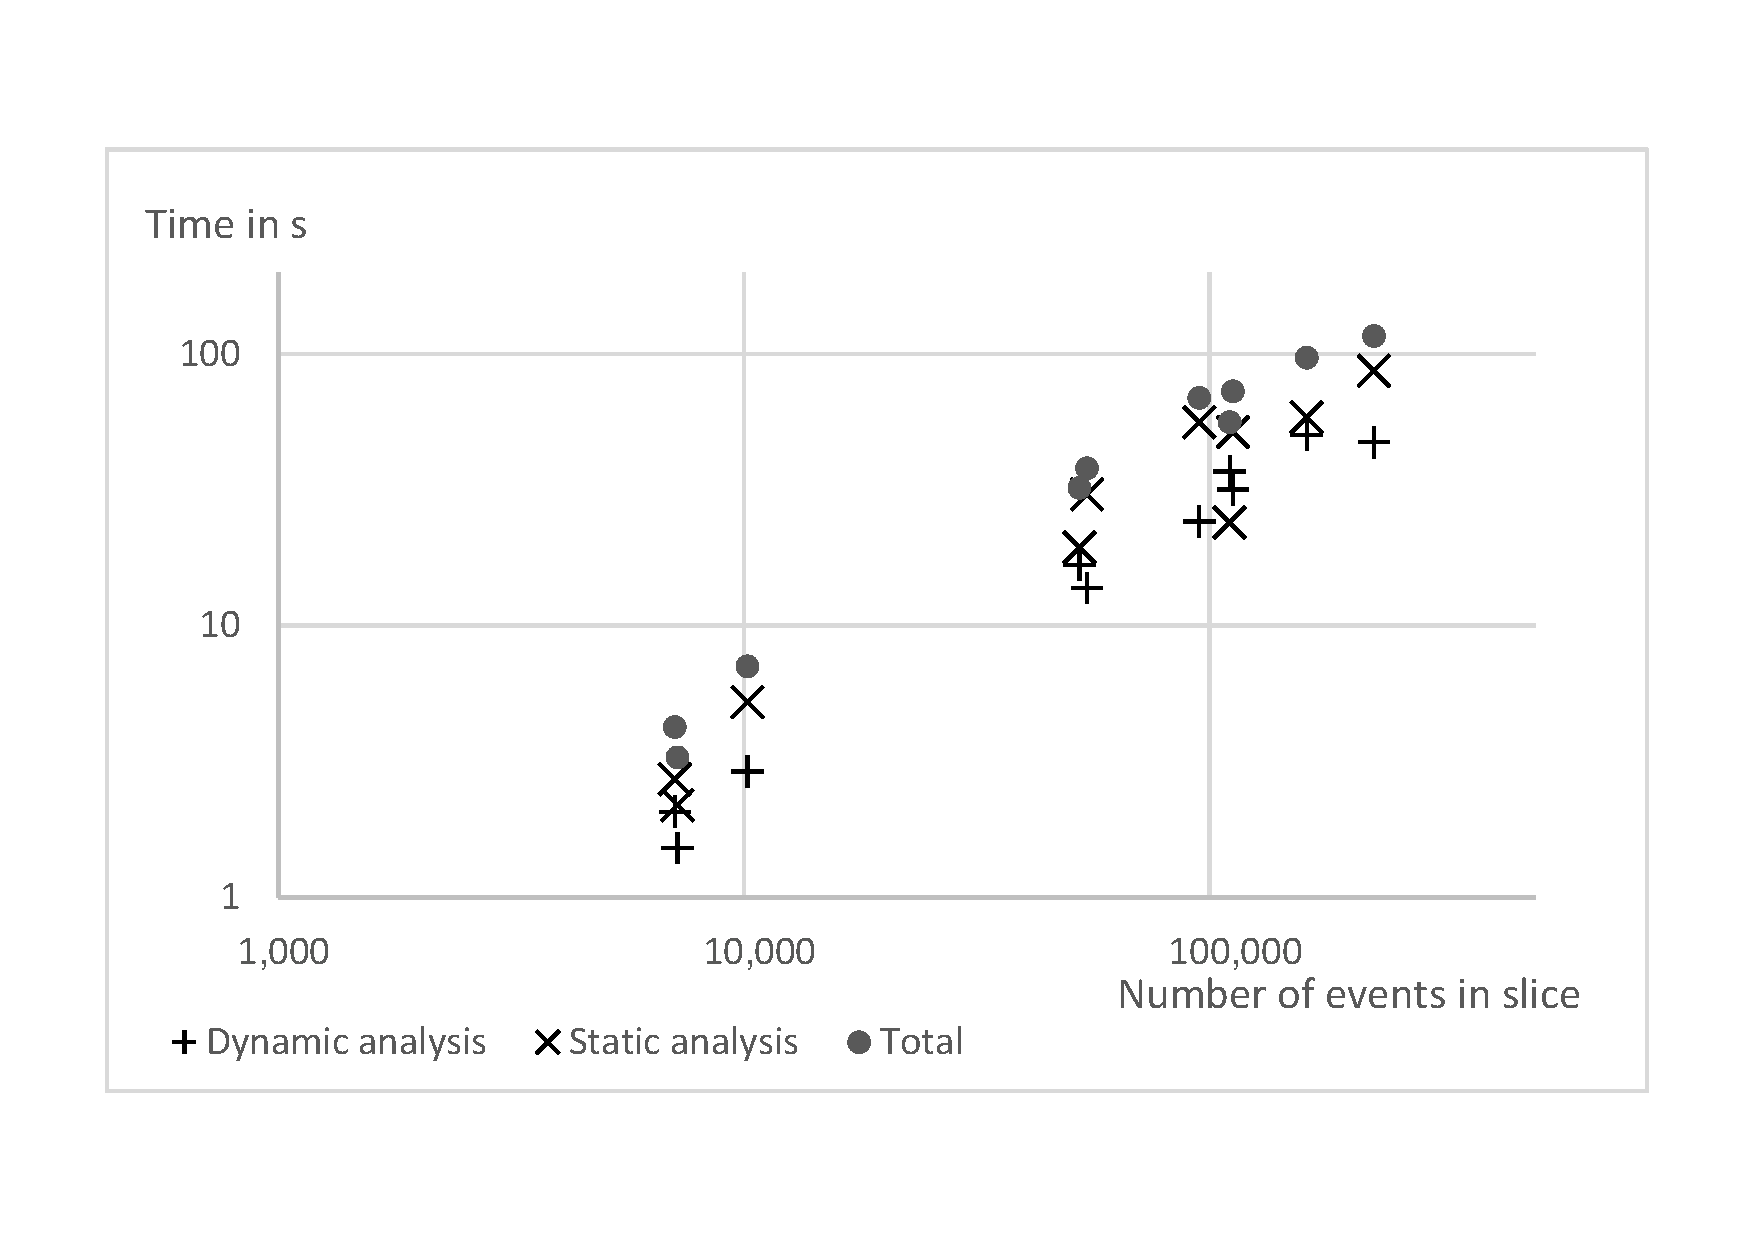
\includegraphics[width=\linewidth, clip, trim={20mm 26mm 20mm 26mm}]{img/chart-initial.pdf}
	\caption{Time for computing the initial slice}
	\label{fig:chartinitial}
\end{figure}

We previously observed that our approach differs from other slicing implementations insofar as that the run-time of the algorithm does not depend on the total length or run-time of the sliced program, but only on the size of the resulting slice~\cite{treffer14:dynamic_slicing_with_soot}.
Our current measurements confirm that slicing time is linear to the result size.

\Cref{fig:chartinitial} shows the time for computing the initial slice in seconds, depending on size of the resulting slice.
Times are given in total, and divided into static code analysis and the dynamic analysis of the event data.

As can be seen, the static analysis takes slightly more time on average.
It should be noted that the total time is less than the sum of the static and dynamic analysis times, as both can, to some extent, run in parallel.
The chart shows that in our setup the algorithm was able to process approximately 1000 events per second.

\begin{figure}
	\centering
		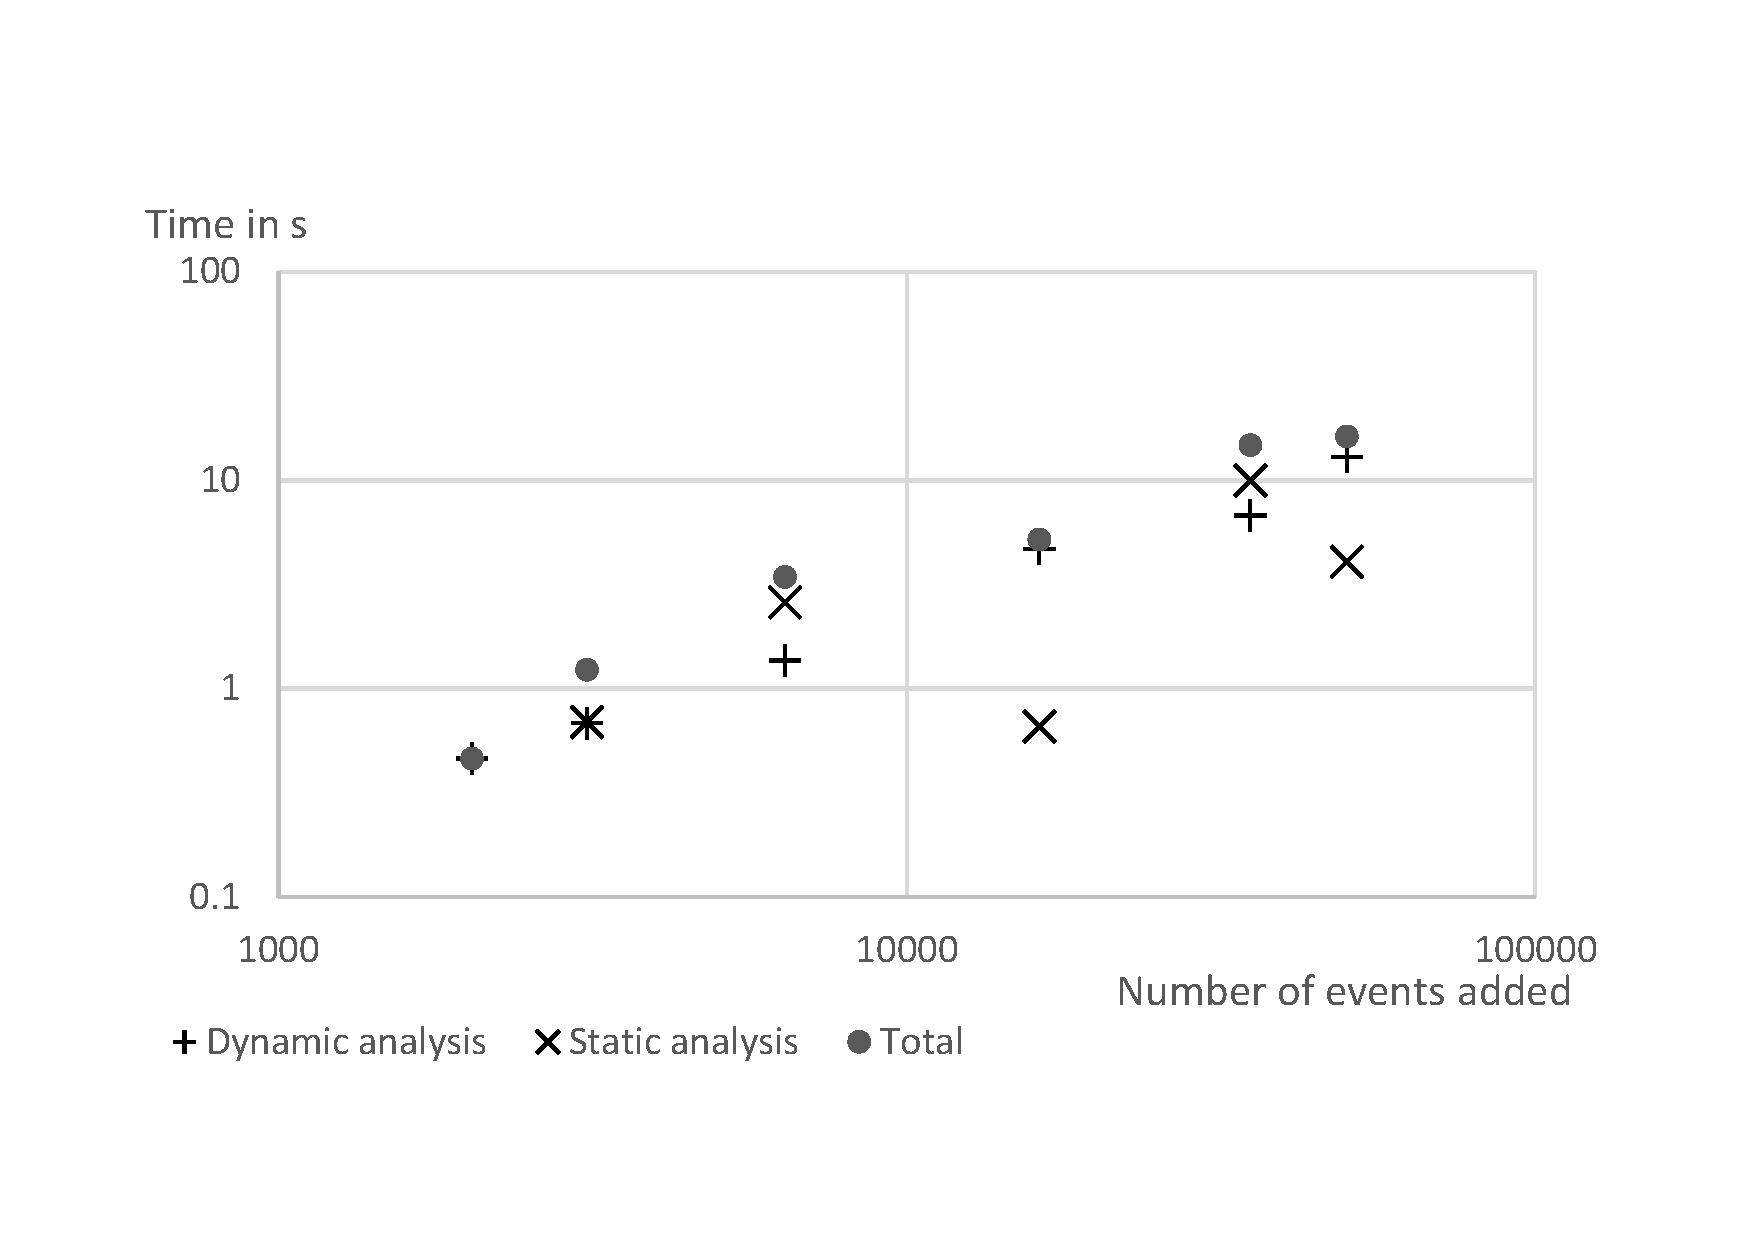
\includegraphics[width=\linewidth, clip, trim={20mm 26mm 20mm 26mm}]{img/chart-add.pdf}
	\caption{Time for adding a slicing criterion}
	\label{fig:chartadd}
\end{figure}

When adding additional elements to the slice, previously computed dependency graphs can be reused.
As \cref{fig:chartadd} shows, the time for dynamic analysis remains constant per event.
The time for static analysis, on the other hand, shows great variation and depends on how much new code was included by the broadened slicing criteria.
In the worst case, expanding the slice takes as long as creating a new slice for only that event.

\begin{figure}
	\centering
		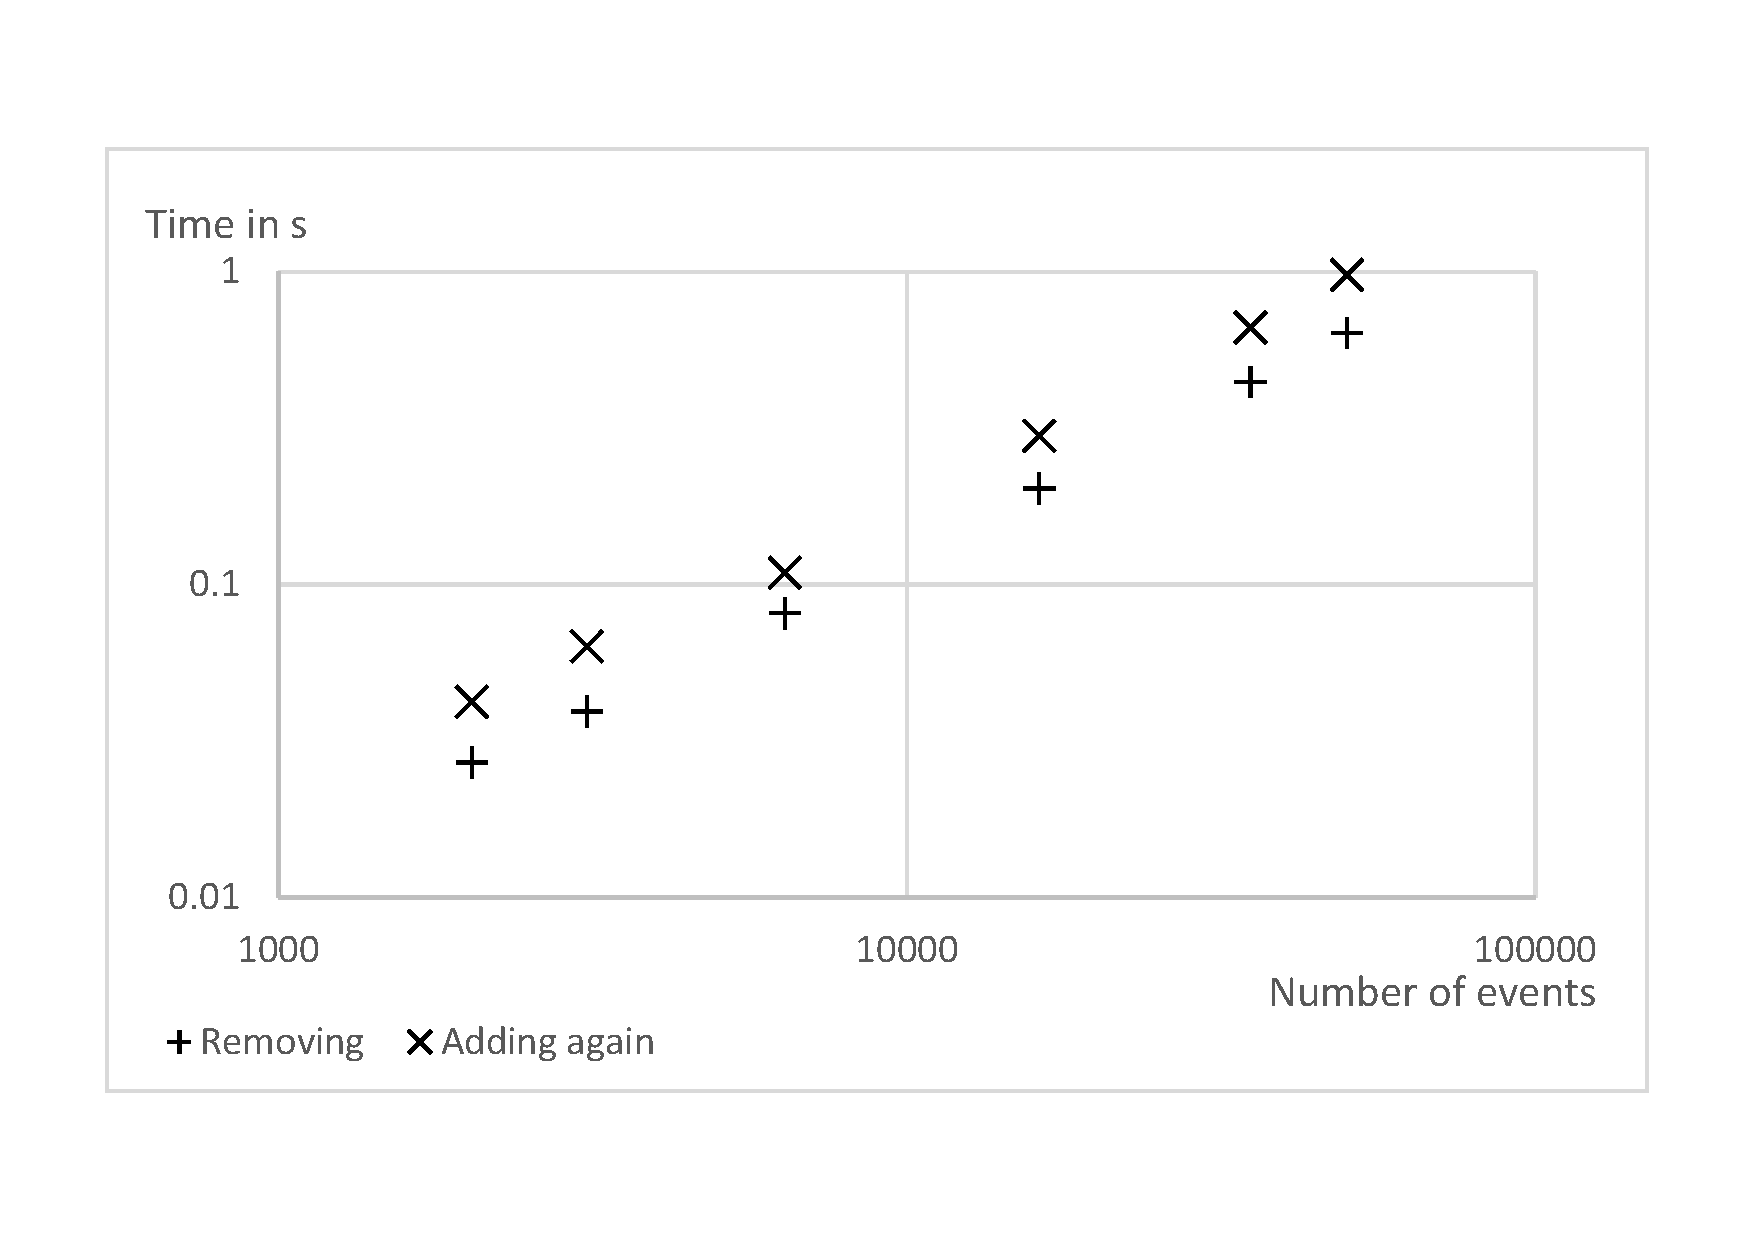
\includegraphics[width=\linewidth, clip, trim={20mm 26mm 20mm 26mm}]{img/chart-rem.pdf}
	\caption{Time for removing events from the slice}
	\label{fig:chartrem}
\end{figure}

\Cref{fig:chartrem} shows that removing events from the slice by narrowing the slicing criteria is significantly faster, as no actual analysis has to be performed.
Likewise, adding those events again by reverting the slicing criteria change is fast, as previously computed dependency graphs can be reused.

\medskip

From the results in \cref{fig:chartinitial}, it seems as if the slicing algorithm is too slow to be of practical use to a developer.
A single second of execution can produce several hundreds of thousands of events and it is generally not feasible to wait multiple minutes for the slicing to complete.
However, due to parallelization and the design of the algorithm, developers experience a delay of only a few seconds.

As described above, the debugging user interface is updated with an intermediate slicing result twice per second.
The slicing algorithm works its way backwards, beginning at the slicing criteria.
Then, previous events are processed not ordered by their absolute position in the execution, but by their distance in the dependency graph.
As a result, both events from the near past and long-running overarching method invocations are processed first.

This allows developers to begin debugging the slice almost immediately. 
From this point on, they can work unimpeded as long as they don't step back faster than the slicer can slice, which is generally given.

For interactive changes of slicing criteria, our experiments have shown that the incremental slicing algorithm is fast enough to not interrupt the developers flow.
In particular, the most common operation -- removing events by narrowing the slicing criteria -- completes in less than a second even for large numbers of events.
From this we conclude that our debugging approach, based on the Slice Navigator and on iterative slice refinements, is generally feasible.

\subsection{User Study}

To gather empirical data on the usefulness of our approach, we conducted an experiment where we let developers locate bugs using a regular debugger, the omniscient debugger from our debugging framework, and the Slice Navigator, and compared their experiences.

\subsubsection{Setup}

We used Defects4J, a database of actual bugs from various open-source projects~\cite{just14:defects4j_a_database}, to find suitable debugging tasks.
For each bug, Defects4J also provides at least one failing test case and the fix.

We chose to conduct the experiment with \emph{Joda Time}\footnote{\url{http://www.joda.org/joda-time/}}, a date and time library for Java, because it has a domain that everyone is already familiar with.
In the version we used for the study, the project contains 68 thousand lines of code in 157 files.
On top of that, there is a test suite of four thousand tests in 154 files, with 69 thousand lines of code.
From the Defects4J bug database, we selected Joda Time bugs 10, 19, and 27.

The bugs were selected because they can be fixed with a small change at a single code location and do not require too much knowledge of the technical details of Joda Time.
Furthermore, all bugs are from different parts of the project, so that the order of the bugs will have no impact on the developers' familiarity with the code in our experiment.
Finally, each bug is caused by a different kind of defect.
We expect that the usefulness of each debugging tool varies depending on the nature of the bug.

The first bug is caused by a wrong hard-coded constant value and documented by a test case that fails with an exception.
From an incorrect variable in the \emph{if}-statement that guards the failure-causing \emph{throw}-statement, developers need to follow the infection chain up to the wrong constant.
The slice for the variable initially contains 324 of the test's 2260 steps.

The second bug is caused by wrongly skipped code, i.e., a too restrictive \textit{if}-condition, and is documented by a test case with a failing assertion.
Again, developers must follow the infection chain, but at some point need to realize the state is now entirely correct and conclude that a value should have been changed at some point.
Slicing on the assertion arguments retains 145 of 465 steps.

The root cause of the third bug is code that gets executed although it should be skipped.
A missing \textit{if}-statement causes a field to be overwritten with a wrong object reference, which leads to wrong code being called via virtual method calls.
Thus, while following the infection chain developers need to realize that wrong code is executed, conclude that a wrong object is used, and then understand why the wrong object was assigned.
Like with the first bug, the test case for bug 3 fails with an exception.
From the incorrect value in the guardian condition of the throw clause, the slice contains 762 of 3190 steps.

We recruited 24 participants for our experiment:
twelve full-time software developers with at least 15 years of programming experience, 
four PhD students in computer science with at least 10 years of programming experience,
and eight computer science graduate students with at least 5 years of programming experience who also worked as programmers in a part-time job for at least one year.
Ages of participants ranged between 25 and 36; two professional developers, one PhD student, and two graduate students were female, all other participants were male.
No participant had previous experience with Joda Time, although 18 participants were aware of its existence.

Every participant was tasked to find the location of each bug by debugging the failing test case with one of the tools.
With the Slice Navigator, we specifically asked the participants not to use the other features of the omniscient debugger and reminded them during the task if necessary.
In the end, every participant had used each tool and every bug was examined with each tool eight times.

For each debugging task, the procedure was as follows:
First, the participant was shown a passing test case similar to the test case they would later have to debug.
We explained the purpose of the test and started the debugging tool to be used.
Then, we let the participant debug the test case, while we explained both the application code and the tool.
When the participant had no more questions, we presented the failing test case and explained the semantics of the failure.
Then we asked the participant to locate the bug using the respective tool and started the timer.
During the debug session, we provided tool support when needed.
If a bug could not be located within 20 minutes, we aborted the task to advance the experiment.

\subsubsection{Comparison of Tool Usage}

\begin{figure}
	\centering
		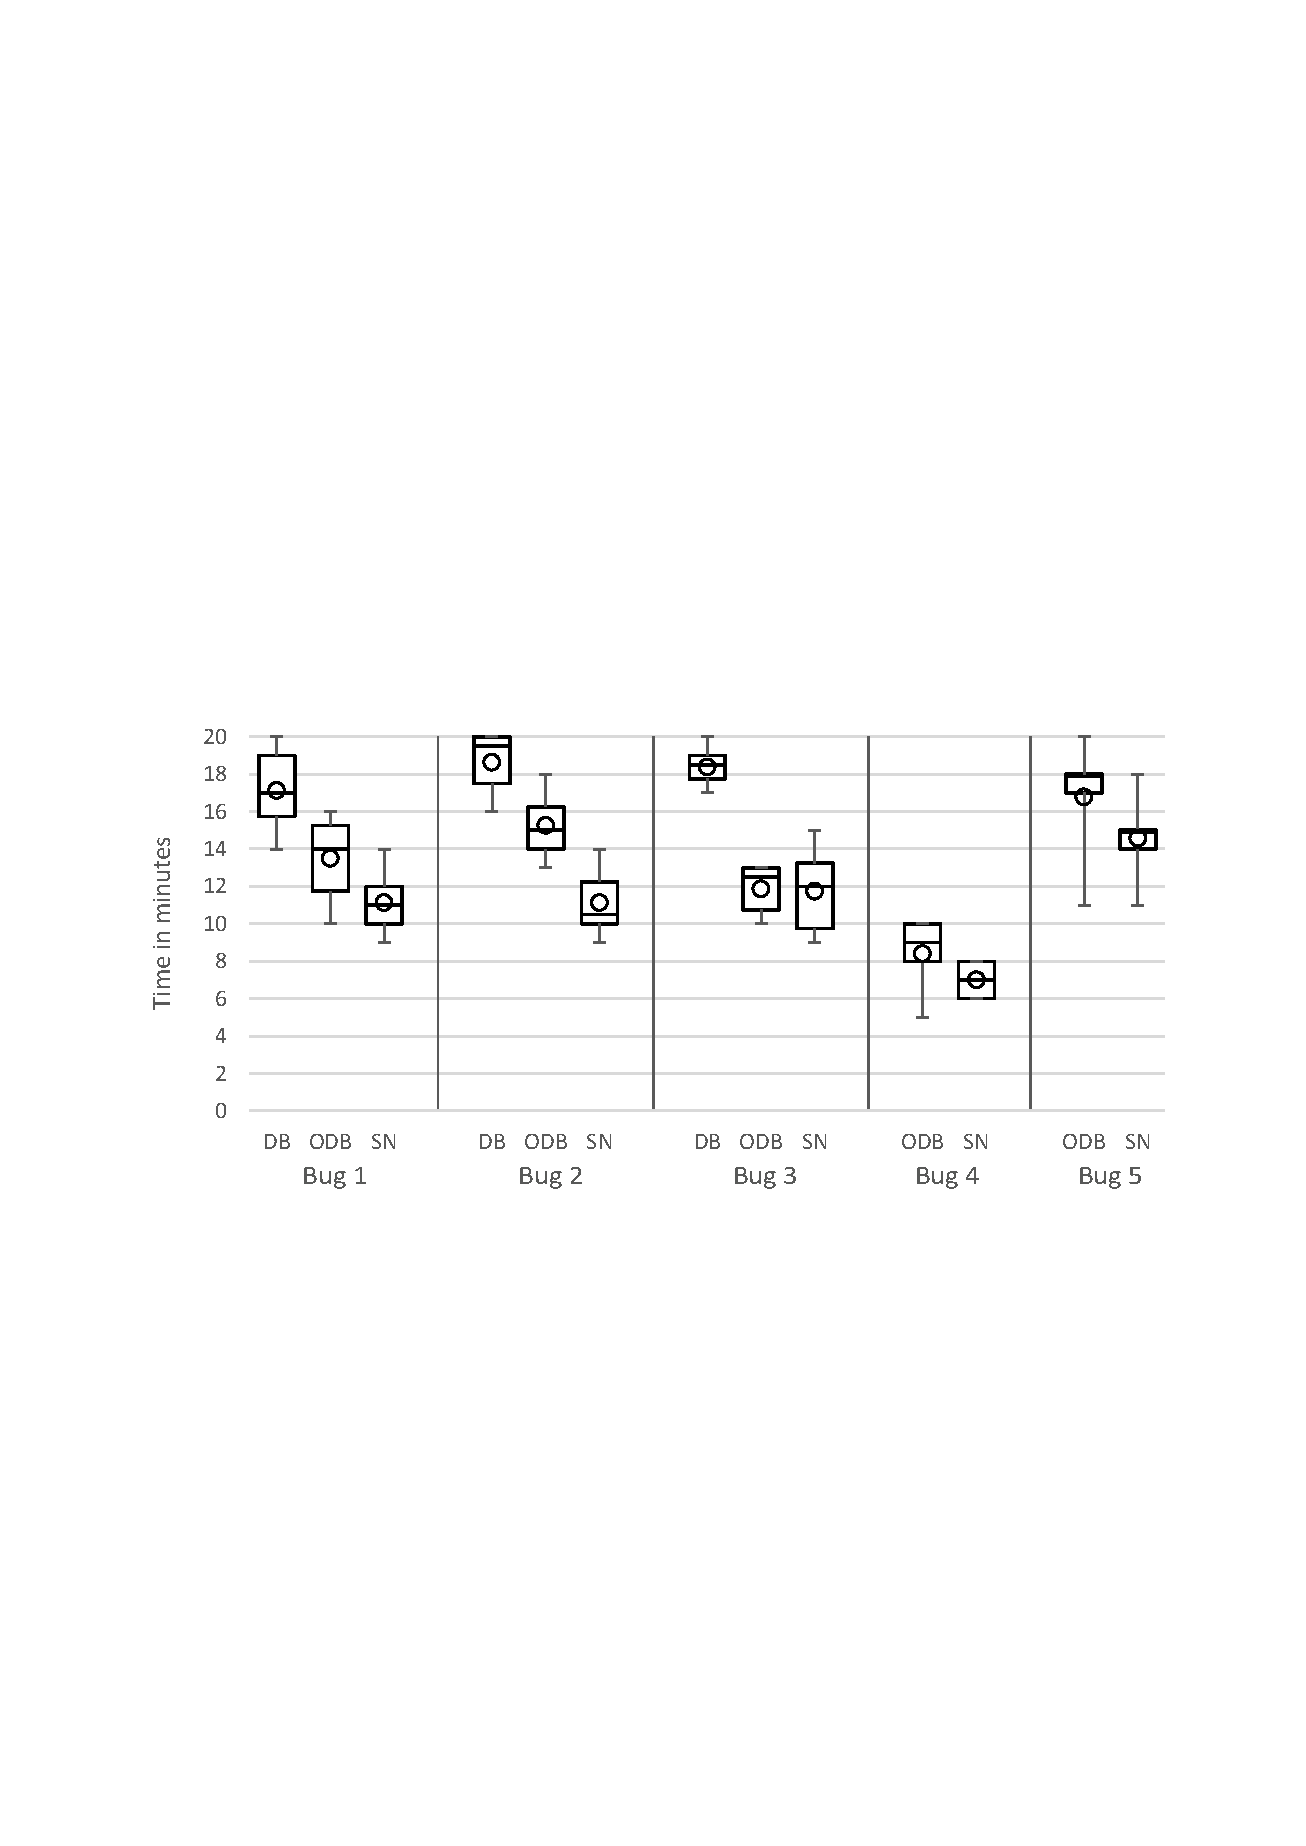
\includegraphics[width=\linewidth]{img/chart-times3.pdf}
	\caption{Time for solving each debugging task with the regular Eclipse Debugger (DB), the omniscient debugger (ODB), and the Slice Navigator (SN)}
	\label{fig:charttimes}
\end{figure}

\Cref{fig:charttimes} shows the time taken for each debugging task in a box plot chart.
Compared to the regular debugger, the Slice Navigator significantly improved the debugging time for each bug.
Relative to the omniscient debugger, developers using the Slice Navigator were faster with two of the three bugs and performed similarly on the third.
Furthermore, we observed changes in developer behavior when using different tools.

With the Eclipse debugger, eight participants made heavy use of the "inspect" feature, which evaluates any expression from the source without further executing the program.
In particular, when contemplating whether to step into or over a method invocation, these participants used "inspect" to preview the invocation result.
The participants who used "inspect" had to restart the debugger on average 3.3($\pm0.8$) times, while the other participants restarted on average 8.4($\pm2.3$) times, and accidentally stepped over a method 2.6($\pm0.9$) times per task.

Furthermore, 10 participants stopped using the debugger entirely for more than a minute, and spent an average of 4.5($\pm1.9$) minutes with pure code reading and mentally simulating the program.
Such behavior was observed with neither of the other two tools.

The omniscient debugger was particularly effective for the third bug, where all but one participants found that a valid field value was overridden by inspecting the object history.
This allowed them to form a good theory about the nature of the bug very early.
However, the method containing the bug is invoked at two different points in time and each time also calls itself recursively.
The bug occurs only in one of the four executions.
With the omniscient debugger, it took developers a while to notice and distinguish the different invocations as they jumped through time.
Overall, with the omniscient debugger developers felt \emph{lost in time} 5.3($\pm1.9$) times per debug session.

Finally, while all developers used the omniscient debugger to step back and forth repeatedly to understand the side effects of a piece of code, 20 of the 24 developers spend most of their time following the infection chain backwards, while four developers mostly debugged forwards in time, like they would with a regular debugger.

With the Slice Navigator, all developers followed the infection chain backwards.
Compared to using only the omniscient debugger, developers were able to reach the end of the infection chain faster, felt lost in time similarly often (on average 5.3($\pm1.9$) times), but took longer to recover from being lost as they had spent less time understanding the code.
However, with the Slice Navigator, developers spent only 1($\pm0.8$) minute per task reading code entirely unrelated to the bug, compared to 4.8($\pm1.5$) minutes with the regular debugger and 3.6($\pm1.6$) minutes with the omniscient debugger.

\subsubsection{Developer Experiences}

After the experiments, we asked the participants how they experienced working with the different tools.

With the omniscient debugger, all participants reported that they found it very helpful to be able to go back and forth in time and felt that they could use it more effectively with more experience, as being used to regular debuggers limited their way of thinking.
Twenty participants said they were at times overwhelmed with the amount of available options and would probably use more of the more advanced features with more experience.
Furthermore, 19 participants expected they would end up lost in time less often with code that they are more familiar with.

For the Slice Navigator, we received similar feedback about moving freely trough time.
Furthermore, all participants liked how the Slice Navigator helped to identify relevant program state.
17 participants perceived this as an improvement in particular to the omniscient debugger, as it was less overwhelming.

However, 11 participants found the overarching dependencies shown in gray to be unnecessary and distracting and emphasized the usefulness of being able to double-click an entry to improve the focus of the slice.
On the other hand, 4 participants said they generally liked the idea of seeing relevant state and would probably find it more useful with code they were more familiar with.

Every participant wrongly clicked or double-clicked an entry at least once and was then unable to recover quickly from the mistake.
Thus, an undo-button was requested by all participants.

Finally, 7 participants reported that while the information provided by the Slice Navigator was very useful, they found it distracted from the actual code.
They liked that with a regular debugger they would rarely have to look away from the code and wished for the slicing context to be visualized within the IDE's code editor.

\subsubsection{Discussion}

Developers that used "inspect" to look ahead in the regular debugger had to restart their debug session less often.
This indicates a general need for moving more freely in time.

While all participants reported they enjoyed working with the Slice Navigator, we received many suggestions for improvement.
Most, like the undo-button or a toggle to hide overarching dependencies, are easily implemented UI features.

Developers getting lost in time reveal a problem that needs further investigation.
This seems to indicate a direction where back-in-time debugging in general can be improved.
The idea of showing the information from the Slice Navigator directly in the code may also help developers to recover from being lost more quickly.

Even though the user interface has still room for improvements, we found a significant improvement in the time needed to locate bugs 1 and 2.

For bug 3, we note that the time needed with the Slice Navigator did not get worse relative to the omniscient debugger, even though we barred users from using the object history view that proved to be very effective for locating this bug.

While the Slice Navigator was not helpful for understanding the root cause in this particular case, it still helped developers to reach the end of the infection chain faster.
Less time and, more importantly, memory was wasted with reading and understanding unrelated code, leading to similar total times.

Overall, the data suggests that the Slice Navigator can make debugging more efficient in many cases.

\subsubsection{Threats to Validity}

External validity is mostly threatened by the size of the study. 
The small number of participants makes it difficult generalize the results.

Likewise, we only considered three bugs from one library.
Although they are real bugs, they all could be tracked down to one location.
For more complex bugs, or bugs in different types of applications, such as web applications, the usefulness of each tool can differ.
To improve the variation, we chose bugs with different characteristics, representing different classes of bugs.

Furthermore, all participants were unfamiliar with the code they had to work with.
Although each participant received an introduction to the code to be debugged, many argued they would have used the tools differently with more familiar code.
A follow-up study should observe programmers using the tools in practice.

Threats to internal validity include the composition of our participant group, which was very heterogeneous with respect to programming experience.
To mitigate this problem, we ensured that participants from each subgroup were distributed evenly across the different debugging tasks.
As \cref{tab:groupresult} shows, students were on average slightly slower using the omniscient debugger and Slice Navigator, but the difference is within the standard deviation of results.
Studies found that computer science students behave very similar to professionals when confronted with new concepts and are therefore suitable for user studies~\cite{host00:using_students_as_subjects, salman15:are_students_representatives}.
However, industry participants appear to use more intuition when identifying important code elements, so some limitations apply~\cite{mcmeekin09:the_significance_of_participant}.

\begin{table}%
	\begin{tabulary}{\textwidth}{LRRR}
		& Eclipse Debugger & Omniscient Debugger & Slice Navigator \\ \midrule
Students & 98\% ($\pm11\%$) & 105\% ($\pm12\%$) & 105\% ($\pm16\%$) \\
Professionals & 102\% ($\pm07\%$) & 95\% ($\pm13\%$) & 95\% ($\pm15\%$) \\
	\end{tabulary}
	\caption{Relative average time taken for debugging tasks with each tool.}
	\label{tab:groupresult}
\end{table}

Internal validity is further threatened by developers gaining experience with the code base throughout the experiment.
We accounted for this by choosing all bugs from different parts of the library, thus achieving the same level of initial knowledge for each task.


\tmpEnd